\documentclass[table,aspectratio=169]{beamer}
%% Choose aspect ratio:
% [aspectratio=43]  % 4:3 (default)
% [aspectratio=169] % 16:9, wide

\usetheme[minimal, nofont, noheadline, nofiles]{tugraz2018}
% \usetheme[iaik,]{tugraz2018}
%% Choose main theme variant:
% [standard]        % standard (default)
% [iaik]       % with institute's graphical acronym on the left
% [minimal]         % with reduced visuals

%% Choose your font style:
%                   % Helvetica (default for Corporate Design)
% [webfont]         % Source Sans Pro (as used on tugraz.at)
% [nofont]          % no font loaded - Computer Modern Sans

%% Choose your department's color instead of TU Graz tugred (optional):
% [arch]            % 
% [bau]             %
% [etit]            %
% [mbww]            %
% [tcvp]            %
% [mpug]            %
% [infbio]          %


\usepackage[utf8]{inputenc}
\usepackage[english]{babel}
%% Choose your language:
% [ngerman]   % German
% [english]   % English


%% Add your own packages, macros, etc.
\usepackage{xcolor,colortbl}
\usepackage{mathtools}
\usepackage{booktabs,nicematrix}
\usepackage{rotating}
\usepackage[style=alphabetic,backend=biber]{biblatex} % Bibliography
\addbibresource{\jobname.bib}                         % Bibliography
\usepackage{fontawesome}
\usepackage{filecontents}
\usepackage{setspace}
\usepackage{mathrsfs}
\usepackage{subcaption}
\usepackage{multirow}
\usepackage{bm}
\usepackage{pgfplots}
\usepackage[linesnumbered,ruled,vlined]{algorithm2e}
\SetKwComment{Comment}{/* }{ */}
\usepackage{framed, color}
\usepackage{tikz}
\usetikzlibrary{external}
\usetikzlibrary{calc,patterns, arrows.meta, shapes.geometric, positioning, decorations.markings, decorations.pathmorphing}
\usetikzlibrary{cipher}
\usepackage{skinny}
\usepackage{tugcolors}
\usepackage{skinnyzero} % definitions for figures: colors, etc
\setbeamersize
{
	text margin left=0.4cm,
	text margin right=0.4cm
}

%% Enter presentation metadata
\title{Automated Methods in Cryptanalysis and Design of Symmetric-Key Cryptographic Primitives}
\author{Hosein Hadipour}
\date{Ph.D. Defense, Graz University of Technology}
%\institute{IAIK}
\instituteurl{hsn.hadipour@gmail.com}

%% Logos
%\institutelogo{beamerthemetugraz/institute/IAIK}  % graphical acronym for [] theme (left margin)
% \additionallogo{figures/logo.jpg}  % additional institute/department logo (footline; optional)
% \logobar{Supported by: ...}  % sponsors (titlepage; optional)


%% Macros
\newcommand{\tikzmark}[1]{\tikz[overlay,remember picture] \node (#1) {};}

\colorlet{upper}{tugred}
\colorlet{upperfix}{tugyellow}
\colorlet{upperunknown}{upper}
\colorlet{lower}{mach}
%\colorlet{lower}{mach} % alternative, brighter mach
\colorlet{lowerfix}{tugmid}
\colorlet{lowerunknown}{lower}
\colorlet{common}{tuggreen}

\newcommand{\dllegupper}[1][black]{\legendwrap{\TFill[#1]{0,0}}}
\newcommand{\dlleglower}[1][black]{\legendwrap{\BFill[#1]{0,0}}}
\newcommand{\dllegend}{%
  \dllegupper[upperfix] active difference
  \dllegupper[upperunknown] unknown difference
  \dlleglower[lowerfix] active mask
  \dlleglower[lowerunknown] unknown mask%
}
\newcommand{\dlshortlegend}{%
  \dllegupper[upper] difference
  \dlleglower[lower] linear mask%
}
\newcommand{\dlfeistellegend}{%
  \tikz[stateopts,baseline=(base)]{\draw[upper,very thick] (0,0) -- (.7,0) ++(0,-.3) coordinate (base);} differential
  \tikz[stateopts,baseline=(base)]{\draw[lower,very thick] (0,0) -- (.7,0) ++(0,-.3) coordinate (base);} linear%
}

\newcolumntype{Y}{>{\centering\arraybackslash}X}
\newcommand{\smallmath}{\everydisplay{\fontsize{8pt}{10pt}\selectfont}}

% S-box tables
\newcommand{\ddt}{\texttt{DDT}\xspace}
\newcommand{\lat}{\texttt{LAT}\xspace}
\newcommand{\bct}{\texttt{BCT}\xspace}
\newcommand{\dlct}{\texttt{DLCT}\xspace}
\newcommand{\udlct}{\texttt{UDLCT}\xspace}
\newcommand{\ldlct}{\texttt{LDLCT}\xspace}
\newcommand{\edlct}{\texttt{EDLCT}\xspace}
\newcommand{\ddlct}{\texttt{DDLCT}\xspace}
\newcommand{\ubct}{\texttt{UBCT}\xspace}
\newcommand{\lbct}{\texttt{LBCT}\xspace}
\newcommand{\ebct}{\texttt{EBCT}\xspace}
\newcommand{\dbct}{\texttt{DBCT}\xspace}
% Correlation and probability
\newcommand{\corr}{\mathbb{C}\xspace}
\newcommand{\pr}{\mathbb{P}\xspace}
\newcommand{\corrmid}{\mathbb{R}\xspace}


% Distinguisher notations
\newcommand{\Up}{_{u}} % Suffix for upper part of the distinguisher
\newcommand{\Mid}{_{m}} % Suffix for middle part of the distinguisher
\newcommand{\Low}{_{\ell}} % Suffix for lower part of the distinguisher
\newcommand{\Dist}{_{D}} % Suffix to represent the distinguisher
\newcommand{\In}{_{\textrm{B}}} % Suffix for inputs
\newcommand{\Out}{_{\textrm{F}}} % Suffix for outputs
\newcommand{\MU}{_{\textsc{mu}}} % Suffix for middle part of the distinguisher
\newcommand{\ML}{_{\textsc{ml}}} % Suffix for middle part of the distinguisher

%%% commands to represent CSP/COP variables/constraints%%%
\newcommand{\ax}{\texttt{AX}\xspace} %AX
\newcommand{\ay}{\texttt{AY}\xspace} %AY
\newcommand{\az}{\texttt{AZ}\xspace} %AZ
\newcommand{\aw}{\texttt{AW}\xspace} %AW
\newcommand{\dx}{\texttt{DX}\xspace} %DX
\newcommand{\lx}{\texttt{LX}\xspace} %LX
\newcommand{\dy}{\texttt{DY}\xspace} %DY
\newcommand{\ly}{\texttt{LY}\xspace} %LY
\newcommand{\dz}{\texttt{DZ}\xspace} %DZ
\newcommand{\lz}{\texttt{LZ}\xspace} %LZ
\newcommand{\dw}{\texttt{DW}\xspace} %DW
\newcommand{\lw}{\texttt{LW}\xspace} %LW
\newcommand{\kx}{\texttt{KX}\xspace} %KX
\newcommand{\ky}{\texttt{KY}\xspace} %KY
\newcommand{\dtk}{\texttt{DTK}\xspace} %DTK
\newcommand{\dstk}{\texttt{DSTK}\xspace} %DSTK

\newcommand{\axu}{\texttt{AXU}\xspace} %AXU
\newcommand{\ayu}{\texttt{AYU}\xspace} %AYU
\newcommand{\azu}{\texttt{AZU}\xspace} %AZU
\newcommand{\dxu}{\texttt{DXU}\xspace} %DXU
\newcommand{\dxmu}{\texttt{DXMU}\xspace} %DXU
\newcommand{\dyu}{\texttt{DYU}\xspace} %DYU
\newcommand{\dzu}{\texttt{DZU}\xspace} %DZU
\newcommand{\lxu}{\texttt{LXU}\xspace} %LXU
\newcommand{\axl}{\texttt{AXL}\xspace} %AXL
\newcommand{\ayl}{\texttt{AYL}\xspace} %AYL
\newcommand{\azl}{\texttt{AZL}\xspace} %AZL
\newcommand{\dxl}{\texttt{DXL}\xspace} %DXL
\newcommand{\dxml}{\texttt{DXML}\xspace} %DXL
\newcommand{\dyl}{\texttt{DYL}\xspace} %DYL
\newcommand{\dzl}{\texttt{DZL}\xspace} %DZL
\newcommand{\lxl}{\texttt{LXL}\xspace} %LXL
\newcommand{\astk}{\texttt{ASTK}\xspace} %ASTK

\newcommand{\xu}{\texttt{XU}\xspace} %XU
\newcommand{\xl}{\texttt{XL}\xspace} %XL
\newcommand{\xmu}{\texttt{XMU}\xspace} %XMU
\newcommand{\xml}{\texttt{XML}\xspace} %XML
\newcommand{\PU}{\texttt{PU}\xspace} %XPU
\newcommand{\QL}{\texttt{QL}\xspace} %CL
\newcommand{\RM}{\texttt{RM}\xspace} %rm

\newcommand{\cp}[1]{\textit{\texttt{#1}}\xspace} % CP x
\newcommand{\csp}{\textit{\texttt{CSP}}\xspace} % CSP problem
\newcommand{\cop}{\textit{\texttt{COP}}\xspace} % COP problem
\newcommand{\cpmodel}{\mathcal{M}\xspace} % CP model M
\newcommand{\cpvars}{\mathcal{M}.\texttt{var}\xspace} % CP variables
\newcommand{\cpcons}{\mathcal{M}.\texttt{con}\xspace} % CP constraints
\newcommand{\cpobj}{\mathcal{M}.\texttt{obj}\xspace} % CP objective
\newcommand{\booltoint}{\textit{\texttt{bool2int}}\xspace} % CP bool2int operator
\newcommand{\cpif}{\textit{\texttt{if}}\xspace} % CP If
\newcommand{\cpthen}{\textit{\texttt{then}}\xspace} % CP Then
\newcommand{\cpelse}{\textit{\texttt{else}}\xspace} % CP Else
\newcommand{\cpelseif}{\textit{\texttt{elseif}}\xspace} % CP Elseif
\newcommand{\cpendif}{\textit{\texttt{endif}}\xspace} % CP Endif

\newcommand{\cplink}{\textit{\texttt{Link}}\xspace} % CP Link
\newcommand{\cpxor}{\textit{\texttt{XOR}}\xspace} % CP XOR
\newcommand{\cpsbox}{\textit{\texttt{S-box}}\xspace} % CP S-box
\newcommand{\cpmds}{\textit{\texttt{MDS}}\xspace} % CP MDS
\newcommand{\cpbranch}{\textit{\texttt{Branch}}\xspace} % CP Branching
\newcommand{\cpcopy}{\textit{\texttt{Copy}}\xspace} % Copy: equivalent to branching point
\newcommand{\cptrue}{\textit{\texttt{True}}\xspace} % CP True
\newcommand{\cpfalse}{\textit{\texttt{False}}\xspace} % CP False
\newcommand{\cplog}{\textit{\texttt{LG}}\xspace} % CP Log(g) - 0.53
\newcommand{\cpmax}{\textit{\texttt{max}}\xspace} % CP Max
\newcommand{\cpmin}{\textit{\texttt{min}}\xspace} % CP Min
\newcommand{\cpmdiff}{\textit{\texttt{Mdiff}}\xspace} % CP Mdiff
\newcommand{\cpminvdiff}{\textit{\texttt{Minvdiff}}\xspace} % CP Minvdiff
\newcommand{\cpmlin}{\textit{\texttt{Mlin}}\xspace} % CP Mlin
\newcommand{\cpminvlin}{\textit{\texttt{Minvlin}}\xspace} % CP Minvlin
\newcommand{\cpmdata}{\textit{\texttt{Mdata}}\xspace} % CP Mdata
\newcommand{\cpminvdata}{\textit{\texttt{Minvdata}}\xspace} % CP Minvdata

\makeatletter
\NewDocumentCommand{\DrawBox}{s O{}}{%
    \tikz[overlay,remember picture]{
    \IfBooleanTF{#1}{%
        \coordinate (RightPoint) at ($(left |- right)+(\linewidth-\labelsep-\labelwidth,0.0)$);
    }{%
        \coordinate (RightPoint) at (right.east);
    }%
    \draw[tugred,#2]
      ($(left)+(-0.2em,0.9em)$) rectangle
      ($(RightPoint)+(0.2em,-0.3em)$);}
}

\NewDocumentCommand{\DrawBoxWide}{s O{}}{%
    \tikz[overlay,remember picture]{
    \IfBooleanTF{#1}{%
        \coordinate (RightPoint) at ($(left |- right)+(\linewidth-\labelsep-\labelwidth,0.0)$);
    }{%
        \coordinate (RightPoint) at (right.east);
    }%
    \draw[tugred,#2]
      ($(left)+(-\labelwidth,0.9em)$) rectangle
      ($(RightPoint)+(0.2em,-0.3em)$);}
}

\def\rowcolor{\noalign{\ifnum0=`}\fi\bmr@rowcolor}
\newcommand<>{\bmr@rowcolor}{%
    \alt#1%
        {\global\let\CT@do@color\CT@@do@color\@ifnextchar[\CT@rowa\CT@rowb}% 
        {\ifnum0=`{\fi}\@gooble@rowcolor}% 
}
\newcommand{\@gooble@rowcolor}[2][]{\@gooble@rowcolor@}
\newcommand{\@gooble@rowcolor@}[1][]{\@gooble@rowcolor@@}
\newcommand{\@gooble@rowcolor@@}[1][]{\ignorespaces}
\newcommand{\sparen}{\vspace*{-.3cm}}

\makeatother

\begin{document}

\begin{frame}[plain]
  \maketitle

  \begin{tikzpicture}[overlay, remember picture]
  % Top image (original photo)
  \node[anchor=south east, xshift=-1.5cm, yshift=1.1cm] at (current page.south east) {
    \begin{tikzpicture}
      \clip (1.5,1.5) circle(1.5cm);
      \includegraphics[width=3cm, height=3cm]{figures/hosein.jpg}; % Original photo
    \end{tikzpicture}
  };
\end{tikzpicture}
\end{frame}

%%%%%%%%%%%%%%%%%%%%%%%%%%%%%%%%%%%%%%%%%%%%%%%%%%%%%%%%%%%%%%%%%%%%%%%%
\begin{frame}[plain]
  \vspace{0.5cm}
  \begin{columns}[T] % Aligns content at the top of each column
    \vspace{0.5cm}
    % First column: Itemized list
    \begin{column}{0.4\textwidth}
      \vbox{
        \begin{itemize}
          \item Special thanks to my advisor, Maria Eichlseder.
          \item I am grateful to my examiners, Gregor Leander and María Naya-Plasencia.  
          \item Thanks to the chair of the deefense meeting, Bernhard Aichernig.
        \end{itemize}
      }
    \end{column}

    % Second column: Images in a triangle layout
    \begin{column}{0.6\textwidth}
      \centering
      \vbox{
        \begin{tikzpicture}
          % Top image - Centered
          \node[anchor=center] at (4.5cm, 7cm) { % Adjusted y-coordinate for more space
            \begin{tikzpicture}
              \node[align=center] {
                \begin{tikzpicture}
                  \clip (1.5,1.5) circle(1.5cm);
                  \includegraphics[width=3cm, height=3cm]{figures/maria.jpg};
                \end{tikzpicture}
                \\ % Line break to place caption below the image
                \textbf{Maria Eichlseder}
              };
            \end{tikzpicture}
          };

          % Bottom-left image
          \node[anchor=center] at (2.2cm, 3.5cm) { % Adjusted x and y coordinates
            \begin{tikzpicture}
              \node[align=center] {
                \begin{tikzpicture}
                  \clip (1.5,1.5) circle(1.5cm);
                  \includegraphics[width=3cm, height=3cm]{figures/marianp.png};
                \end{tikzpicture}
                \\ % Line break to place caption below the image
                \textbf{María Naya-Plasencia}
              };
            \end{tikzpicture}
          };

          % Bottom-right image
          \node[anchor=center] at (6.8cm, 3.5cm) { % Adjusted x and y coordinates
            \begin{tikzpicture}
              \node[align=center] {
                \begin{tikzpicture}
                  \clip (1.5,1.5) circle(1.5cm);
                  \includegraphics[width=3cm, height=3cm]{figures/gregor.png};
                \end{tikzpicture}
                \\ % Line break to place caption below the image
                \textbf{Gregor Leander}
              };
            \end{tikzpicture}
          };
        \end{tikzpicture}
      }
    \end{column}
  \end{columns}
\end{frame}

%%%%%%%%%%%%%%%%%%%%%%%%%%%%%%%%%%%%%%%%%%%%%%%%%%%%%%%%%%%%%%%%%%%%%%%%
\section*{}
\begin{frame}{Outline}
  \tableofcontents
\end{frame}

%%%%%%%%%%%%%%%%%%%%%%%%%%%%%%%%%%%%%%%%%%%%%%%%%%%%%%%%%%%%%%%%%%%%%%%%
\section{Research Gaps and Thesis Contributions}
\sectionheader[\huge\color{tugblue}\faBinoculars/\color{tug}\faDiamond]{Research Gaps and Thesis Contributions}

%%%%%%%%%%%%%%%%%%%%%%%%%%%%%%%%%%%%%%%%%%%%%%%%%%%%%%%%%%%%%%%%%%%%%%%%
\begin{frame}{Challenges and Gaps}
Automated cryptanalysis has advanced significantly in the past decade, \textbf{yet}:
\begin{itemize}
\item[\color{tugblue}{\faBinoculars}] Accuracy and efficiency of current methods remain suboptimal.
\item[\color{tugblue}{\faBinoculars}] Many cryptanalytic techniques were not (fully) automated before this work. %, e.g., guess-and-dtermine, impossible differential, integral, and differential-linear attacks. 
\item[\color{tugblue}{\faBinoculars}] New cryptanalytic techniques demand novel automation tools. 
\item[\color{tugblue}{\faBinoculars}] Emerging primitives necessitate new methodologies for automated cryptanalysis.
\item[\color{tugblue}{\faBinoculars}] The connections between attacks are not well used in automated discovery.
\end{itemize}
\end{frame}

%%%%%%%%%%%%%%%%%%%%%%%%%%%%%%%%%%%%%%%%%%%%%%%%%%%%%%%%%%%%%%%%%%%%%%%%
\begin{frame}{Our Contributions/Publications -- I}
\begin{itemize}
\footnotesize
\item[\faDiamond] \fullcite{mine_acns_HadipourE22}
\item[\faDiamond] \fullcite{tosc_HadipourE22}
\item[\faDiamond] \fullcite{tosc_HadipourNE22}
\end{itemize}
\end{frame}

\begin{frame}{Our Contributions/Publications -- II}
\begin{itemize}
\footnotesize
\item[\faDiamond] \fullcite{eurocrypt_HadipourSE23}
\item[\faDiamond] \fullcite{zeroplus_cryptoeprint_2023_1701}
\item[\faDiamond] \fullcite{journals_tosc_HadipourT24}
\end{itemize}
\end{frame}

\begin{frame}{Our Contributions/Publications -- III}
\begin{itemize}
\footnotesize
\item[\faDiamond] \fullcite{crypto_HDE2024}
\item[\color{tugblue}{\faDiamond}] \fullcite{tosc_ChakrabortyHNM24}
\item[\color{tugblue}{\faDiamond}] \fullcite{journals_tches_SoleimanyBHRBM22}
\end{itemize}
\end{frame}

%%%%%%%%%%%%%%%%%%%%%%%%%%%%%%%%%%%%%%%%%%%%%%%%%%%%%%%%%%%%%%%%%%%%%%%%
\section{Background}
\sectionheader[\huge\color{tug}\faBook]{Background}

%%%%%%%%%%%%%%%%%%%%%%%%%%%%%%%%%%%%%%%%%%%%%%%%%%%%%%%%%%%%%%%%%%%%%%%%
\begin{frame}{Cryptography -- Primary Goals}
\vspace{-0.6cm}
\begin{figure}
\centering
\begin{tikzpicture}[scale=0.4]

  \tikzstyle{every node}=[transform shape];

  % Alice
  \node (label) at (0,0) {\includegraphics[height=7cm]{figures/canal_alice_dep.pdf}};
  \node (label) at (0,-4) {\Huge\bf Alice};
  
  % Bob
  \node (label) at (30,0) {\includegraphics[height=7cm]{figures/canal_bob_dep.pdf}};
  \node (label) at (30,-4) {\Huge\bf Bob};

  % Eve
  \node (label) at (15,-6) {\includegraphics[height=7cm]{figures/canal_eve_dep.pdf}};
  \node (label) at (15,-10) {\Huge\bf Eve};
  \draw[->, line width=1mm, rounded corners=2pt] (12,-7) -- ++(-3,0) -- node[left] {\Huge\bf \textcolor{tugred}{Listen}} ++(0,+5.5);
  \draw[->, line width=1mm, rounded corners=2pt] (18,-7) -- ++(+3,0) --  node[right] {\Huge\bf \textcolor{tugblue}{Manipulate}} ++(0,+5.5);

  % Canal
  \draw[line width=1mm] (4,-1) ellipse (0.7 and 1);
  \draw[line width=1mm] (25,-2) arc (-90:90:1);

  \draw[line width=1mm] (4,0) -- ++(21,0);
  \draw[line width=1mm] (4,-2) -- ++(21,0);
  \node (label) at (14.5, 0.5) {\Huge Insecure Channel};
\end{tikzpicture}
\end{figure}
\vspace{-0.2cm} % Push content to the bottom
\hspace*{\fill}%
1- \textbf{\textcolor{tugred}{Confidentiality}} %
\hspace{\fill}%
2- \textbf{\textcolor{tugblue}{Integrity}} %
\hspace{\fill}%
3- \textbf{Authentication} %
\hspace*{\fill}%
\end{frame}

%%%%%%%%%%%%%%%%%%%%%%%%%%%%%%%%%%%%%%%%%%%%%%%%%%%%%%%%%%%%%%%%%%%%%%%%
\begin{frame}[plain]{}%{{{
  %\tikzsetnextfilename{primitives-lockview}
  \begin{tikzpicture}[remember picture, overlay]
    \fill[dark] (current page.north west) rectangle (current page.south east);
    \begin{scope}[scale=4, shift=(current page.center), very thick]
      \draw[white, line width=1ex, rounded corners=2ex, fill]
        (0,-.55) +(-1,-.5) rectangle +(1,1);
      \draw[white, line width=5.0ex] (0,-.55) +(-.6,1) arc (180:0:.6);

      \coordinate (mid) at (0,-.300);
      %\pause
      \node[box, draw, very thick, minimum width=6.25cm, minimum height=4.5cm] (protocols) at ($(mid)+(0,-.15)$) {};
      \draw (protocols.north west) node[above right] {Protocols \color{black!45}\footnotesize -- TLS, \dots};
      \pause
      \node[box, draw, very thick, minimum width=4.5cm, minimum height=3cm] (schemes) at ($(mid)+(0,-.25)$) {};
      \draw (schemes.north west) node[above right] {\!Schemes \vphantom{p}\color{black!45}\footnotesize -- AES-GCM, \dots};
      \pause
      \only<1-4>{\node[box, draw, very thick, minimum width=2.85cm, minimum height=1.5cm, white] (primitives) at ($(mid)+(0,-.35)$) {};}
      \only<5>{\node[box, draw, very thick, minimum width=2.85cm, minimum height=1.5cm, yellow] (primitives) at ($(mid)+(0,-.35)$) {};}
      \draw (primitives.north west) node[above right] {Primitives \color{black!45}\footnotesize -- AES, \dots};
      \draw[box, font=\color{white}, minimum size=.5cm] (mid) ++(0,-.38)
                                                       +(   0,0) node[fill=tug] (E2) {}
                                                       +(-.25,0) node[fill=tug] (E1) {}
                                                       +( .25,0) node[fill=tug] (E3) {};
      % \pause
      \only<beamer:4|handout:1>{
          \foreach \i in {1,2,3} {
            \draw[next] (E\i) ++ (0,.25*.75) -- (E\i);
          }
          \draw[next] (E1) ++(-.25*.75,0) -- (E1);
          \draw[next] (E1) -- (E2);
          \draw[next] (E2) -- (E3);
          \draw[next] (E3) -- ++(.25*.75,0);
          %\coordinate (E1) ++(0,-.85) {};
      }
    \end{scope}
  \end{tikzpicture}
\end{frame}%}}}

%%%%%%%%%%%%%%%%%%%%%%%%%%%%%%%%%%%%%%%%%%%%%%%%%%%%%%%%%%%%%%%%%%%%%%%%
\begin{frame}{Cryptographic Primitives}
\vspace{-0.6cm}
\begin{itemize}
\item Symmetric-Key Primitives
\vspace{-0.25cm}
\begin{itemize}
\footnotesize
\item Block ciphers (AES \cite{daemen1999aes}, CLEFIA \cite{conf_fse_ShiraiSAMI07})
\item Tweakable block ciphers (SKINNY \cite{skinny_spec}, QARMAv2 \cite{qarmav2_spec})
\item Unkeyed primitives (Ascon \cite{ascon_jocDobraunigEMS21, asconnist}, Keccak \cite{eurocrypt_BertoniDPA13})
\item Stream ciphers (Trivium \cite{canniere2008trivium}, ZUC \cite{zuc128_specification}, Enocoro-128v2 \cite{watanabe2010hardware})
\end{itemize}
\vspace{-0.3cm}
\item Public-Key Primitives
\begin{itemize}
\vspace{-0.25cm}
\footnotesize
\item Public-key encryption algorithms (RSA, ECC)
\item Digital signature algorithms (RSA, ECC)
\item Key-exchange algorithms (DH)
\end{itemize}
\vspace{-0.25cm}
\item \textcolor{tuggreen}{\textbf{Hybrid Approach}}
\end{itemize}
\vspace{-2.5cm}
\hfill
\includegraphics[width=0.3\textwidth]{./figures/tls.png}
\end{frame}

%%%%%%%%%%%%%%%%%%%%%%%%%%%%%%%%%%%%%%%%%%%%%%%%%%%%%%%%%%%%%%%%%%%%%%%%
% {
% \newcommand{\PT}{\strut$P$\,\faFileTextO}%
% \newcommand{\CT}{\strut$C$\,\faEnvelopeO}%\faFileText \faEnvelope
% \newcommand{\K}{\strut$K$\,\faKey}%
% \newcommand{\T}{\strut$T$\,\faPaperclip}%\faFileCodeO \faTag \faPaperclip
% \newcommand{\D}[1]{\strut$#1$\,\faDatabase}
% \begin{frame}[c]{Symmetric Primitives}%{{{
%     %\tikzsetnextfilename{primitives-types}
%     \centering
%     \begin{tikzpicture}[yscale=1, xscale=1, thick,
%                         every node/.style={inner sep=1pt},
%                         next/.append style={rounded corners=3pt},
%                         primi/.append style={fill=main, minimum width=1cm, minimum height=1cm, draw=white, rounded corners=2pt},
%                         caption/.style={gray, below=1.75cm, align=center}]
%       \node[primi, key west] (E) {$E$};
%       \draw[next]  (E) ++ (0,1) node[above] {\PT} -- (E);
%       \draw[next]  (E) ++(-1,1) node[above] {\K } |- (E);
%       \draw[prev]  (E) ++(0,-1) node[below] {\CT} -- (E);
%       \node[caption] at (E) {Block Cipher\\(BC)};

%       \node[primi, key west] (ET) at (4,0) {$\tilde{E}$};
%       %\node[primi, key west] (ET) at (4,0) {$\tilde{E}$};
%       \draw[next]  (ET) ++ (0,1) node[above] {\PT} -- (ET);
%       \draw[next]  (ET) ++ (1,1) node[above] {\T } |- (ET);
%       \draw[next]  (ET) ++(-1,1) node[above] {\K } |- (ET);
%       \draw[prev]  (ET) ++(0,-1) node[below] {\CT} -- (ET);
%       \node[caption] at (ET) {Tweakable BC\\(TBC)};

%       \node[primi, minimum width=1.25cm]
%                    (EP) at (8,0) {$P$};
%       \draw[next]  (EP) ++ (0,1) node[above] {\D{X}} -- (EP);
%       \draw[prev]  (EP) ++(0,-1) node[below] {\D{Y}} -- (EP);
%       \node[caption] at (EP) {Permutation};

%       \node[primi, minimum width=1cm, shape=compression]
%                    (EC) at (12,0) {$F$};
%                    %(EC) at (12,0) {$F$};
%       \draw[next]  (EC) ++ (-.5,1) node[above] (X1) {\D{Z}} -- (EC.north-|X1);
%       \draw[next]  (EC) ++ ( .5,1) node[above] (X2) {\D{X}} -- (EC.north-|X2);
%       \draw[prev]  (EC) ++(0,-1) node[below] {\D{Y}} -- (EC);
%       \node[caption] at (EC) {Compression\\Function};

%       %\node at (14.5,0) {\faEllipsisH};
%       %\node at (10.5,0) {\faEllipsisH};
%     \end{tikzpicture}
% \end{frame}
% }%}}}

%%%%%%%%%%%%%%%%%%%%%%%%%%%%%%%%%%%%%%%%%%%%%%%%%%%%%%%%%%%%%%%%%%%%%%%%
\begin{frame}{Overview of Block Cipher Designs}
\vbox{
% Top half: left and right parts
\hbox{
\parbox[b]{0.15\textwidth}{%
\centering % topleft
\begin{tikzpicture}[yscale=1, xscale=1, thick,
                    every node/.style={inner sep=1pt},
                    next/.append style={rounded corners=3pt},
                    primi/.append style={fill=main, minimum width=1cm, minimum height=1cm, draw=white, rounded corners=2pt},
                    caption/.style={gray, below=1.75cm, align=center}]
  \node[primi, key west] (E) {$E$};
  \draw[next]  (E) ++ (0,1) node[above] {$P$} -- (E);
  \draw[next]  (E) ++(-1,1) node[above] {$K$} |- (E);
  \draw[prev]  (E) ++(0,-1) node[below] {$C$} -- (E);
  % \node[caption] at (E) {Block Cipher\\(BC)};
\end{tikzpicture}
}
% \hfill
\parbox[b]{0.85\textwidth}{%
\centering % topright
\resizebox{0.75\textwidth}{!}{
\begin{tikzpicture}[xscale=1,yscale=1,very thin,>=latex]
\coordinate (here) at (0, 0);
\node[xor, right=1cm of here] (AK) {};
\node[box, right=0.5cm of AK] (R) {$\bm{f}_1$};
\coordinate[above=1.5cm of AK] (RKSource);
\node[right=1cm of R] (DOTS){$\cdots$};
\draw[next] (here) -- (AK);
\coordinate (T1) at ($(AK.north) + (-0.5, 1.5)$) {};
\coordinate (T4) at ($(AK.north) + (0.5, 2.2)$) {};
\coordinate (K0_1) at ($(AK.north) + (-1.15, 1.85)$);
\coordinate (K0_2) at ($(AK.north) + (0, 1.85)$);
\node[] at ($(here) + (0.25, -0.31)$) {$P$};
\draw[next] (AK) -- (R);
\draw[next] (R) -- (DOTS);
\node[] at ($(R) + (0.92, -0.31)$) {$X_{1}$};
\draw[next] (RKSource) -- node[anchor=east] {$K_{1}$} (AK);
\draw[fill opacity = 1, rounded corners=1mm, dashed] ($(here) + (0.78, -0.5)$) rectangle ($(here) + (2.65, 0.55)$) node[below, midway, yshift=-0.5cm] {$\bm{F}_1$};
\coordinate[right=1pt of DOTS] (here);
\draw[next, rounded corners=1mm] (K0_1) -- node[above] {$K$} (K0_2);

\node[xor, right=1cm of here] (AK) {};
\node[box, right=0.5cm of AK] (R) {$\bm{f}_{i}$};
\coordinate[above=1.5cm of AK] (RKSource);
\node[right=1cm of R] (DOTS){$\cdots$};
\draw[next] (here) -- (AK);
\node[] at ($(here) + (0.25, -0.31)$) {$X_{i - 1}$};
\draw[next] (AK) -- (R);
\draw[next] (R) -- (DOTS);
\node[] at ($(R) + (0.92, -0.31)$) {$X_{i}$};
\draw[next] (RKSource) -- node[anchor=east] {$K_{i}$} (AK);
\draw[fill opacity = 1, rounded corners=1mm, dashed] ($(here) + (0.78, -0.5)$) rectangle ($(here) + (2.65, 0.55)$) node[below, midway, yshift=-0.5cm] {$\bm{F}_i$};
\coordinate[right=1pt of DOTS] (here);

\node[xor, right=1cm of here] (AK) {};
\node[box, right=0.5cm of AK] (R) {$\bm{f}_{r}$};
\coordinate[above=1.5cm of AK] (RKSource);
\node[right=0.6cm of R] (DOTS){};
\node[right=0.35cm of DOTS] (cipher){};
\coordinate (T2) at ($(AK.north) + (2.5, 1.5)$) {};
\coordinate (T3) at ($(AK.north) + (1.5, 2.2)$) {};
\draw[next] (here) -- (AK);
\node[next] at ($(here) + (0.25, -0.31)$) {$X_{r - 1}$};
\draw[next] (AK) -- (R);
\draw[next] (R) -- (DOTS);
\draw[next] (DOTS) -- (cipher);
\node[xor] (ALK) at (DOTS) {};
\coordinate[above=1.5cm of ALK] (LRKSource);
\node[] at ($(R) + (0.92, -0.31)$) {$X_{r}$};
\node[] at ($(R) + (1.5, -0.31)$) {$C$};
\draw[next] (RKSource) -- node[anchor=east] {$K_{r}$} (AK);
\draw[next] (LRKSource) -- node[anchor=east] {$K_{r + 1}$} (ALK);
\draw[fill opacity = 1, rounded corners=1mm, dashed] ($(here) + (0.78, -0.5)$) rectangle ($(here) + (2.65, 0.55)$) node[below, midway, yshift=-0.5cm] {$\bm{F}_r$};
\draw[rounded corners=1mm] (T1) -- (T2) -- (T3) -- (T4) -- cycle;
\node[above=0.1cm of $(T1)!0.5!(T2)$] {Key Schedule};
\end{tikzpicture}}
}
}
\vspace{0.2cm}
% Bottom half
\parbox[b]{\textwidth}{%
\centering % bottom
\includegraphics[width=0.85\textwidth]{./figures/aes_round_function.pdf}
}
}
\end{frame}

%%%%%%%%%%%%%%%%%%%%%%%%%%%%%%%%%%%%%%%%%%%%%%%%%%%%%%%%%%%%%%%%%%%%%%%%
\begin{frame}{Cryptanalysis}
\vspace{-0.5cm}
\begin{itemize}
  \item \textbf{Information-Theoretic Approach}
  \begin{itemize}
    \item Provides generic bounds for security against unconditional adversaries
  \end{itemize}

  \item \textbf{Complexity-Theoretic Approach}
  \begin{itemize}
    \item Based on reduction techniques
    \item More common in public-key cryptography
  \end{itemize}

  \item \textbf{\textcolor{tugred}{Cryptanalytic Approach}}
  \begin{itemize}
    \item Evaluates security against concrete known attacks
    \item More common in symmetric-key cryptography
  \end{itemize}
\end{itemize}
\end{frame}

%%%%%%%%%%%%%%%%%%%%%%%%%%%%%%%%%%%%%%%%%%%%%%%%%%%%%%%%%%%%%%%%%%%%%%%%
\begin{frame}{Well-Known Cryptanalytic Attacks}
\vspace{-0.5cm}
\begin{itemize}
  \small
  \item \textcolor{tugred}{Differential attack} \cite{crypto_BihamS90} (Full round DES \cite{crypto_BihamS92}/AES-256 \cite{crypto_BiryukovKN09})
  \item \textcolor{tugred}{Linear attack} \cite{eurocrypt_Matsui93} (Full round DES \cite{eurocrypt_Matsui93}) 
  \item \textcolor{tugred}{Boomerang attack} \cite{fse_Wagner99} (Full round COCONUT98 \cite{fse_Wagner99})
  \item \textcolor{tugred}{Differential-Linear (DL) attack} \cite{dl_crypto_LangfordH94} (Full round COCONUT98 \cite{enhanced_dl_asiacrypt_BihamDK02})
  \item \textcolor{tugred}{Impossible-Differential (ID) attack} \cite{knudsen1998deal, eurocrypt_BihamBS99} (7 rounds of AES)
  \item \textcolor{tugred}{Integral attack} \cite{Lai1994, square_fse_DaemenKR97} (Full-round \cipher{MISTY1}~\cite{crypto_Todo15})
  \item \textcolor{tugred}{Cube attack} \cite{eurocrypt_DinurS09} (Best attack type on SHA-3 \cite{eurocrypt_HuangWXWZ17})
  \item And some others, e.g., zero-correlation (ZC), meet-in-the-middle attacks. 
\end{itemize}
\end{frame}

%%%%%%%%%%%%%%%%%%%%%%%%%%%%%%%%%%%%%%%%%%%%%%%%%%%%%%%%%%%%%%%%%%%%%%%%
\begin{frame}{Automated Methods in Cryptanalysis}
\textbf{Mounting cryptanalytic attacks against symmetric-key primitives:}
\begin{itemize}
  \item Requires tracing the propagation of a certain property at the bit-level
  \item Implies solving a hard combinatorial optimization problem
  \item Is very time-consuming
  \item Is potentially an error-prone process
\end{itemize}

\vspace{-0.4cm}
\begin{block}{Automated Methods in Cryptanalysis}
Leveraging machines to \textcolor{tugred}{\textbf{find}}, \textcolor{tugblue}{\textbf{build}}, or \textcolor{tuggreen}{\textbf{optimize}} cryptanalytic attacks.
\end{block}
\end{frame}

%%%%%%%%%%%%%%%%%%%%%%%%%%%%%%%%%%%%%%%%%%%%%%%%%%%%%%%%%%%%%%%%%%%%%%%%
\begin{frame}{Different Approaches for Automatic Cryptanalysis}
\vspace{-0.5cm}
\begin{itemize}
\item Dedicated algorithms
\item {\color<1>{tugred} \textbf{Constraint Programming (CP)}}
\begin{itemize}
\item {\color<1>{tugred} Satistifiability (SAT)}
\item {\color<1>{tugred} Satistifiability Modulo Theories (SMT)}
\item {\color<1>{tugred} Mixed Integer Linear Programming (MILP)}
\item {\color<1>{tugred} Constraint Satisfaction/Optimization Problem (CSP/COP)}
\end{itemize}
\item Artificial Intelligence (AI)
\end{itemize}
\end{frame}

%%%%%%%%%%%%%%%%%%%%%%%%%%%%%%%%%%%%%%%%%%%%%%%%%%%%%%%%%%%%%%%%%%%%%%%%
\begin{frame}{Constraint Programming (CP)}
\begin{itemize}
% \item Programming in CP refers to the arrangement of a plan
% \item For example the \href{https://developers.google.com/optimization/scheduling/employee_scheduling}{employee scheduling problem}
\item Constraint Satisfaction/Optimization Problem (CSP/COP):
\begin{itemize}
\item We define a set of variables: $\mathcal{X} = \{\mathcal{X}_{1}, \ldots, \mathcal{X}_{n}\}$
\item We specify the domain of each variable: $\mathbb{F}_{2}, \mathbb{Z}, \mathbb{R}, \ldots$
\item We define a set of constraints: $\mathcal{C} = \{\mathcal{C}_{1}, \ldots, \mathcal{C}_{2}\}$
\item We define an objective function (if it is required)
\end{itemize}
\item Constraint Programming (CP): Searching for a solution for a CSP/COP
\item \textcolor{tugred}{MILP} and \textcolor{tugblue}{SMT/SAT} are special cases of CP
\end{itemize}
\end{frame}


%%%%%%%%%%%%%%%%%%%%%%%%%%%%%%%%%%%%%%%%%%%%%%%%%%%%%%%%%%%%%%%%%%%%%%%%
\begin{frame}[fragile]
\frametitle{Constraint Programming -- Example I}
\begin{columns}
\column[c]{0.45\textwidth}
\begin{center}
\only<1>{\includegraphics[width=0.9\textwidth]{./figures/austria.pdf}}
\only<2>{\includegraphics[width=0.9\textwidth]{./figures/austria_legend.pdf}}
\only<3>{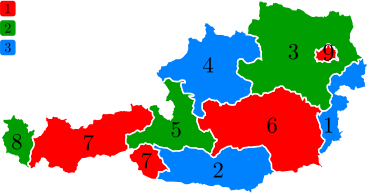
\includegraphics[width=0.9\textwidth]{./figures/austria3colored.pdf}}
\end{center}
\column[c]{0.55\textwidth}
\pause
{\scriptsize
\begin{verbatim}
int: NC = 3;
array[1..9] of var 1..NC: R;
constraint R[1] != R[3]; constraint R[1] != R[6];
constraint R[2] != R[5]; constraint R[2] != R[6]; 
constraint R[2] != R[7]; constraint R[3] != R[9]; 
constraint R[3] != R[6]; constraint R[3] != R[4];
constraint R[4] != R[6]; constraint R[4] != R[5];
constraint R[5] != R[6]; constraint R[5] != R[7];
constraint R[7] != R[8];
solve satisfy;
\end{verbatim}}
\pause
\vspace{-0.2cm}
\color{tuggreen}{
{\scriptsize
\begin{verbatim}
R = [3, 3, 2, 3, 2, 1, 1, 2, 1];
\end{verbatim}}}
\end{columns}
\end{frame}

%%%%%%%%%%%%%%%%%%%%%%%%%%%%%%%%%%%%%%%%%%%%%%%%%%%%%%%%%%%%%%%%%%%%%%%%
% \begin{frame}{Challenges and Gaps}
% Automated cryptanalysis has advanced significantly in the past decade, \textbf{yet}:
% \begin{itemize}
% \item Accuracy and efficiency of current methods remain suboptimal.
% \item Many cryptanalytic techniques were not (fully) automated before this work, e.g., guess-and-dtermine, impossible differential, integral, and differential-linear attacks. 
% \item New cryptanalytic techniques demand novel automation tools. 
% \item Emerging primitives necessitate new methodologies for automated cryptanalysis.
% \end{itemize}
% \end{frame}

%%%%%%%%%%%%%%%%%%%%%%%%%%%%%%%%%%%%%%%%%%%%%%%%%%%%%%%%%%%%%%%%%%%%%%%%
\section{Automated Tools for Impossible-Differential, Zero-Correlation and Integral Attacks}
\sectionheader[\huge\color{tug}\faLightbulbO\faLightbulbO\faLightbulbO]{Automated Tools for Impossible-Differential, \\Zero-Correlation and Integral Attacks}

%%%%%%%%%%%%%%%%%%%%%%%%%%%%%%%%%%%%%%%%%%%%%%%%%%%%%%%%%%%%%%%%%%%%%%%%
\begin{frame}[fragile]{Integral, ID, and ZC Distinguishers}
\vspace{-1cm}
\begin{columns}[onlytextwidth]
\column[c]{0.6\textwidth}
\begin{itemize}
\small
\item<1-> Integral attack \cite{hod_discrete_derivatives_lai1994higher, square_fse_DaemenKR97}
% \begin{itemize}
%   \item Partial-sum technique \cite{fseFergusonKLSSWW00}
% \end{itemize}
\item<3-> Impossible-differential attack \cite{eurocrypt_BihamBS99, knudsen1998deal}
% \begin{itemize}
%   \item Early abort technique \cite{ctrsa_LuKKD08}
% \end{itemize}
\item<4-> Zero-correlation attack \cite{dcc_BogdanovR14}
\end{itemize}
\column[c]{0.4\textwidth}
\begin{center}
\begin{overprint}
\begin{tikzpicture}[yscale=1, xscale=1, thick,
every node/.style={inner sep=5pt},
next/.append style={rounded corners=3pt},
primi/.append style={fill=tugred!50, draw=black, rounded corners=2pt, minimum size=30pt},
caption/.style={gray, below=1.75cm, align=center}]
\pgfmathsetmacro{\cubex}{1.5}
\pgfmathsetmacro{\cubey}{1.5}
\pgfmathsetmacro{\cubez}{1.5}

\visible<2>{
\draw[tuggray,fill=tugblue!50,opacity=0.5] (0.5,+2.5,0) -- ++(-\cubex,0,0) -- ++(0,-\cubey,0) -- ++(\cubex,0,0) -- cycle;
\draw[tuggray,fill=tugblue!50,opacity=0.5] (0.5,+2.5,0) -- ++(0,0,-\cubez) -- ++(0,-\cubey,0) -- ++(0,0,\cubez) -- cycle;
\draw[tuggray,fill=tugblue!50] (0.5,+2.5,0) -- ++(-\cubex,0,0) -- ++(0,0,-\cubez) -- ++(\cubex,0,0) -- cycle;
}

\node[primi, key east] (E) {$E$};
\draw[next]  (E) ++(0,1.5) node[above, name=x] {$\bm{x}$\,\faFileTextO} -- (E);
\draw[next]  (E) ++(+1,0) node[above, name=k]{$\bm{k}$\,\faKey} -- (E);
\draw[prev]  (E) ++(0,-1.5) node[below, name=y] {
\only<1>{$\bm{y}$\,\faEnvelopeO}
\only<2>{\textcolor{tugred}{\bgroup\smallmath$\textcolor{tugred}{\sum_{x \in \bm{x}} \bm{y} = 0}$\egroup}}
\only<3->{$\bm{y}$\,\faEnvelopeO}
} -- (E);

\visible<3>{
\node[primi, key west, left=1.2cm of E] (E) {$E$};
\draw[next]  (E) ++(0,1.5) node[above, name=xp] {\faFileText\,$\bm{x'}$} -- (E);
\draw[next]  (E) ++(-1,0) node[above, name=kp] {$\bm{k}$\,\faKey} -- (E);
\draw[prev]  (E) ++(0,-1.5) node[below, name=yp] {\faEnvelope\,$y'$} -- (E);
\draw[<->, dashed] (x) -- node[above, name=dp] {$\Delta x$} (xp);
\draw[<->, dashed] (y) -- node[above, name=dc] {$\Delta y$} (yp);
\node[below=0.2cm of dc] {\textcolor{tugred}{$\Pr(\Delta\bm{x} \rightarrow \Delta\bm{y}) = 0$}};
}

\visible<4>{
\draw[->, dashed] (x) -- node[above] {$\cdot \bm{\lambda}_{i}$} (xp);
\draw[->, dashed] (y) -- node[above] {$\cdot \bm{\lambda}_{o}$} (yp); 
\node at (xp) {$\bm{\lambda}_{i} \cdot \bm{x}$};
\node at (yp) {$\bm{\lambda}_{o} \cdot \bm{y}$};
% \draw[->, dashed] (xp) -- node[left=0.2cm, rotate=90] {\scriptsize $\bm{\lambda}_{i}\cdot \bm{x} \oplus \bm{\lambda}_{o}\cdot \bm{y}$} (yp);
\draw[->, dashed] (xp) -- (yp);
\node[below=0.2cm of dc] {\footnotesize \textcolor{tugred}{$\bm{Corr}(\bm{\lambda}_{i}\cdot \bm{x} \oplus \bm{\lambda}_{o}\cdot \bm{y}) = 0$}}; 
}

\end{tikzpicture}
\end{overprint}
\end{center}
\end{columns}
\end{frame}


%%%%%%%%%%%%%%%%%%%%%%%%%%%%%%%%%%%%%%%%%%%%%%%%%%%%%%%%%%%%%%%%%%%%%%%%
% \begin{frame}{\cipher{SKINNY} Family of Tweakable Block Ciphers \cite{skinny}}
% \begin{figure}
% \centering
% \begin{tikzpicture}[cellopts/.append style={font=\scriptsize}, xscale=1.05, yscale=1.1]
%   \SkinnyInit{}{}{}{}
%   \SkinnyRoundTK[r] % round number
%                 {\Cell{s0} {\ttfamily 0}\Cell{s1} {\ttfamily 1}\Cell{s2} {\ttfamily 2}\Cell{s3} {\ttfamily 3}
%                   \Cell{s4} {\ttfamily 4}\Cell{s5} {\ttfamily 5}\Cell{s6} {\ttfamily 6}\Cell{s7} {\ttfamily 7}
%                   \Cell{s8} {\ttfamily 8}\Cell{s9} {\ttfamily 9}\Cell{s10}{\ttfamily a}\Cell{s11}{\ttfamily b}
%                   \Cell{s12}{\ttfamily c}\Cell{s13}{\ttfamily d}\Cell{s14}{\ttfamily e}\Cell{s15}{\ttfamily f}}
%                 {\fill[gray!15] (ss00) ++(-.5,.5) rectangle +(4,-2);}{}{} % tk[1,2,3]
%                 {\fill[gray!15] (ss00) ++(-.5,.5) rectangle +(4,-2);} % states (after subcells)
%                 {\fill[gray!15] (ss00) ++(-.5,.5) rectangle +(4,-2);}{} % states (after addtweakey, shiftrows)

%   \SkinnyFin[r+1]{}
% \end{tikzpicture}
% \end{figure}
% \begin{itemize}
%   \small
%   \item Introduced in CRYPTO~2016 \cite{skinny}
%   \item It has 6 main variants: \cipher{SKINNY}-$n$-$z\cdot\!n$, where $n\in \{64, 128\}$, and $z\in \{1, 2, 3\}$
%   \item ISO/IEC 18033-7: \cipher{SKINNY}-64-192, \cipher{SKINNY}-128-256, \cipher{SKINNY}-128-384
% \end{itemize}
% \end{frame}

%%%%%%%%%%%%%%%%%%%%%%%%%%%%%%%%%%%%%%%%%%%%%%%%%%%%%%%%%%%%%%%%%%%%%%%
\begin{frame}{Miss-in-the-Middle Technique \cite{eurocrypt_BihamBS99}}
\vspace{-0.7cm}
\begin{itemize}
\small
\item Find two differences (linear masks) that propagate forward and backward with probability one and contradict each other in the middle
\end{itemize}

\begin{figure}
\vspace{-0.5cm}
\centering
\resizebox{0.9\linewidth}{!}{
\begin{tikzpicture}[xscale=1.1, yscale=1.1]
\SkinnyInit{}{}{}{} % init coordinates, print labels

\SkinnyRoundTK[0]
      {\visible<2->{\FillCell[white]{s0}\FillCell[white]{s1}\FillCell[nonzeroany]{s2}\FillCell[nonzeroany]{s3}\FillCell[white]{s4}\FillCell[white]{s5}\FillCell[white]{s6}\FillCell[white]{s7}\FillCell[white]{s8}\FillCell[white]{s9}\FillCell[white]{s10}\FillCell[white]{s11}\FillCell[nonzeroany]{s12}\FillCell[white]{s13}\FillCell[white]{s14}\FillCell[nonzeroany]{s15}}} % state (input)
      {\Cell{s0}{\texttt{0}}\Cell{s1}{\texttt{1}}\Cell{s2}{\texttt{2}}\Cell{s3}{\texttt{3}}\Cell{s4}{\texttt{4}}\Cell{s5}{\texttt{5}}\Cell{s6}{\texttt{6}}\Cell{s7}{\texttt{7}}} % tk[1]
      {} % tk[2]
      {} % tk[3]
      {\visible<3->{\FillCell[white]{s0}\FillCell[white]{s1}\FillCell[nonzeroany]{s2}\FillCell[nonzeroany]{s3}\FillCell[white]{s4}\FillCell[white]{s5}\FillCell[white]{s6}\FillCell[white]{s7}\FillCell[white]{s8}\FillCell[white]{s9}\FillCell[white]{s10}\FillCell[white]{s11}\FillCell[nonzeroany]{s12}\FillCell[white]{s13}\FillCell[white]{s14}\FillCell[nonzeroany]{s15}}} % state (after subcells)
      {\visible<4->{\FillCell[white]{s0}\FillCell[white]{s1}\FillCell[nonzeroany]{s2}\FillCell[nonzeroany]{s3}\FillCell[white]{s4}\FillCell[white]{s5}\FillCell[white]{s6}\FillCell[white]{s7}\FillCell[white]{s8}\FillCell[white]{s9}\FillCell[white]{s10}\FillCell[white]{s11}\FillCell[nonzeroany]{s12}\FillCell[white]{s13}\FillCell[white]{s14}\FillCell[nonzeroany]{s15}}} % state (after addtweakey)
      {\visible<5->{\FillCell[white]{s0}\FillCell[white]{s1}\FillCell[nonzeroany]{s2}\FillCell[nonzeroany]{s3}\FillCell[white]{s5}\FillCell[white]{s6}\FillCell[white]{s7}\FillCell[white]{s4}\FillCell[white]{s10}\FillCell[white]{s11}\FillCell[white]{s8}\FillCell[white]{s9}\FillCell[nonzeroany]{s15}\FillCell[white]{s12}\FillCell[white]{s13}\FillCell[nonzeroany]{s14}}} % state (after shiftrows)

\SkinnyRoundTK[1]
      {\visible<6->{\FillCell[white]{s0}\FillCell[white]{s1}\FillCell[unknown]{s2}\FillCell[unknown]{s3}\FillCell[white]{s4}\FillCell[white]{s5}\FillCell[nonzeroany]{s6}\FillCell[nonzeroany]{s7}\FillCell[white]{s8}\FillCell[white]{s9}\FillCell[white]{s10}\FillCell[white]{s11}\FillCell[white]{s12}\FillCell[white]{s13}\FillCell[nonzeroany]{s14}\FillCell[nonzeroany]{s15}}} % state (input)
      {\Cell{s0}{\texttt{9}}\Cell{s1}{\texttt{f}}\Cell{s2}{\texttt{8}}\Cell{s3}{\texttt{d}}\Cell{s4}{\texttt{a}}\Cell{s5}{\texttt{e}}\Cell{s6}{\texttt{c}}\Cell{s7}{\texttt{b}}} % tk[1]
      {} % tk[2]
      {} % tk[3]
      {\visible<7->{\FillCell[white]{s0}\FillCell[white]{s1}\FillCell[unknown]{s2}\FillCell[unknown]{s3}\FillCell[white]{s4}\FillCell[white]{s5}\FillCell[nonzeroany]{s6}\FillCell[nonzeroany]{s7}\FillCell[white]{s8}\FillCell[white]{s9}\FillCell[white]{s10}\FillCell[white]{s11}\FillCell[white]{s12}\FillCell[white]{s13}\FillCell[nonzeroany]{s14}\FillCell[nonzeroany]{s15}}} % state (after subcells)
      {\visible<8->{\FillCell[white]{s0}\FillCell[white]{s1}\FillCell[unknown]{s2}\FillCell[unknown]{s3}\FillCell[white]{s4}\FillCell[white]{s5}\FillCell[nonzeroany]{s6}\FillCell[nonzeroany]{s7}\FillCell[white]{s8}\FillCell[white]{s9}\FillCell[white]{s10}\FillCell[white]{s11}\FillCell[white]{s12}\FillCell[white]{s13}\FillCell[nonzeroany]{s14}\FillCell[nonzeroany]{s15}}} % state (after addtweakey)
      {\visible<9->{\FillCell[white]{s0}\FillCell[white]{s1}\FillCell[unknown]{s2}\FillCell[unknown]{s3}\FillCell[white]{s5}\FillCell[white]{s6}\FillCell[nonzeroany]{s7}\FillCell[nonzeroany]{s4}\FillCell[white]{s10}\FillCell[white]{s11}\FillCell[white]{s8}\FillCell[white]{s9}\FillCell[white]{s15}\FillCell[white]{s12}\FillCell[nonzeroany]{s13}\FillCell[nonzeroany]{s14}}} % state (after shiftrows)

\SkinnyNewLine[2]{\visible<10->{\FillCell[white]{s0}\FillCell[nonzeroany]{s1}\FillCell[unknown]{s2}\FillCell[unknown]{s3}\FillCell[white]{s4}\FillCell[white]{s5}\FillCell[unknown]{s6}\FillCell[unknown]{s7}\FillCell[nonzeroany]{s8}\FillCell[white]{s9}\FillCell[white]{s10}\FillCell[nonzeroany]{s11}\FillCell[white]{s12}\FillCell[white]{s13}\FillCell[unknown]{s14}\FillCell[unknown]{s15}}} % state (after mixcols)
\SkinnyRoundTK[2]
      {\visible<11->{\FillCell[white]{s0}\FillCell[nonzeroany]{s1}\FillCell[unknown]{s2}\FillCell[unknown]{s3}\FillCell[white]{s4}\FillCell[white]{s5}\FillCell[unknown]{s6}\FillCell[unknown]{s7}\FillCell[nonzeroany]{s8}\FillCell[white]{s9}\FillCell[white]{s10}\FillCell[nonzeroany]{s11}\FillCell[white]{s12}\FillCell[white]{s13}\FillCell[unknown]{s14}\FillCell[unknown]{s15}}} % state (input)
      {\Cell{s0}{\texttt{1}}\Cell{s1}{\texttt{7}}\Cell{s2}{\texttt{0}}\Cell{s3}{\texttt{5}}\Cell{s4}{\texttt{2}}\Cell{s5}{\texttt{6}}\Cell{s6}{\texttt{4}}\Cell{s7}{\texttt{3}}} % tk[1]
      {} % tk[2]
      {} % tk[3]
      {\visible<12->{\FillCell[white]{s0}\FillCell[nonzeroany]{s1}\FillCell[unknown]{s2}\FillCell[unknown]{s3}\FillCell[white]{s4}\FillCell[white]{s5}\FillCell[unknown]{s6}\FillCell[unknown]{s7}\FillCell[nonzeroany]{s8}\FillCell[white]{s9}\FillCell[white]{s10}\FillCell[nonzeroany]{s11}\FillCell[white]{s12}\FillCell[white]{s13}\FillCell[unknown]{s14}\FillCell[unknown]{s15}}} % state (after subcells)
      {\visible<13->{\FillCell[white]{s0}\FillCell[nonzeroany]{s1}\FillCell[unknown]{s2}\FillCell[unknown]{s3}\FillCell[white]{s4}\FillCell[white]{s5}\FillCell[unknown]{s6}\FillCell[unknown]{s7}\FillCell[nonzeroany]{s8}\FillCell[white]{s9}\FillCell[white]{s10}\FillCell[nonzeroany]{s11}\FillCell[white]{s12}\FillCell[white]{s13}\FillCell[unknown]{s14}\FillCell[unknown]{s15}}} % state (after addtweakey)
      {\visible<14->{\FillCell[white]{s0}\FillCell[nonzeroany]{s1}\FillCell[unknown]{s2}\FillCell[unknown]{s3}\FillCell[white]{s5}\FillCell[white]{s6}\FillCell[unknown]{s7}\FillCell[unknown]{s4}\FillCell[nonzeroany]{s10}\FillCell[white]{s11}\FillCell[white]{s8}\FillCell[nonzeroany]{s9}\FillCell[white]{s15}\FillCell[white]{s12}\FillCell[unknown]{s13}\FillCell[unknown]{s14}}} % state (after shiftrows)

\SkinnyMismatchAligned[3]{\visible<15->{\FillCell[white]{s0}\FillCell[unknown]{s1}\FillCell[unknown]{s2}\FillCell[unknown]{s3}\FillCell[white]{s4}\FillCell[nonzeroany]{s5}\FillCell[unknown]{s6}\FillCell[unknown]{s7}\FillCell[unknown]{s8}\FillCell[nonzeroany]{s9}\FillCell[nonzeroany]{s10}\FillCell[unknown]{s11}\FillCell[white]{s12}\FillCell[unknown]{s13}\FillCell[unknown]{s14}\FillCell[unknown]{s15}}} % state (after mixcols)
\SkinnyRoundTK[3]
      {\visible<15->{\FillCell[nonzeroany]{s0}\FillCell[unknown]{s1}\FillCell[unknown]{s2}\FillCell[unknown]{s3}\FillCell[unknown]{s4}\FillCell[unknown]{s5}\FillCell[unknown]{s6}\FillCell[unknown]{s7}\FillCell[unknown]{s8}\FillCell[unknown]{s9}\FillCell[unknown]{s10}\FillCell[unknown]{s11}\FillCell[unknown]{s12}\FillCell[unknown]{s13}\FillCell[unknown]{s14}\FillCell[unknown]{s15}}} % state (input)
      {\Cell{s0}{\texttt{f}}\Cell{s1}{\texttt{b}}\Cell{s2}{\texttt{9}}\Cell{s3}{\texttt{e}}\Cell{s4}{\texttt{8}}\Cell{s5}{\texttt{c}}\Cell{s6}{\texttt{a}}\Cell{s7}{\texttt{d}}} % tk[1]
      {} % tk[2]
      {} % tk[3]
      {\visible<14->{\FillCell[nonzeroany]{s0}\FillCell[unknown]{s1}\FillCell[unknown]{s2}\FillCell[unknown]{s3}\FillCell[unknown]{s4}\FillCell[unknown]{s5}\FillCell[unknown]{s6}\FillCell[unknown]{s7}\FillCell[unknown]{s8}\FillCell[unknown]{s9}\FillCell[unknown]{s10}\FillCell[unknown]{s11}\FillCell[unknown]{s12}\FillCell[unknown]{s13}\FillCell[unknown]{s14}\FillCell[unknown]{s15}}} % state (after subcells)
      {\visible<13->{\FillCell[nonzeroany]{s0}\FillCell[unknown]{s1}\FillCell[unknown]{s2}\FillCell[unknown]{s3}\FillCell[unknown]{s4}\FillCell[unknown]{s5}\FillCell[unknown]{s6}\FillCell[unknown]{s7}\FillCell[unknown]{s8}\FillCell[unknown]{s9}\FillCell[unknown]{s10}\FillCell[unknown]{s11}\FillCell[unknown]{s12}\FillCell[unknown]{s13}\FillCell[unknown]{s14}\FillCell[unknown]{s15}}} % state (after addtweakey)
      {\visible<12->{\FillCell[nonzeroany]{s0}\FillCell[unknown]{s1}\FillCell[unknown]{s2}\FillCell[unknown]{s3}\FillCell[unknown]{s5}\FillCell[unknown]{s6}\FillCell[unknown]{s7}\FillCell[unknown]{s4}\FillCell[unknown]{s10}\FillCell[unknown]{s11}\FillCell[unknown]{s8}\FillCell[unknown]{s9}\FillCell[unknown]{s15}\FillCell[unknown]{s12}\FillCell[unknown]{s13}\FillCell[unknown]{s14}}} % state (after shiftrows)

\SkinnyNewLine[3]{\visible<11->{\FillCell[unknown]{s0}\FillCell[white]{s1}\FillCell[unknown]{s2}\FillCell[unknown]{s3}\FillCell[nonzeroany]{s4}\FillCell[unknown]{s5}\FillCell[unknown]{s6}\FillCell[unknown]{s7}\FillCell[unknown]{s8}\FillCell[unknown]{s9}\FillCell[unknown]{s10}\FillCell[nonzeroany]{s11}\FillCell[unknown]{s12}\FillCell[unknown]{s13}\FillCell[unknown]{s14}\FillCell[unknown]{s15}}} % state (after mixcols)
\SkinnyRoundTK[3]
      {\visible<10->{\FillCell[unknown]{s0}\FillCell[white]{s1}\FillCell[unknown]{s2}\FillCell[unknown]{s3}\FillCell[nonzeroany]{s4}\FillCell[unknown]{s5}\FillCell[unknown]{s6}\FillCell[unknown]{s7}\FillCell[unknown]{s8}\FillCell[unknown]{s9}\FillCell[unknown]{s10}\FillCell[nonzeroany]{s11}\FillCell[unknown]{s12}\FillCell[unknown]{s13}\FillCell[unknown]{s14}\FillCell[unknown]{s15}}} % state (input)
      {\Cell{s0}{\texttt{7}}\Cell{s1}{\texttt{3}}\Cell{s2}{\texttt{1}}\Cell{s3}{\texttt{6}}\Cell{s4}{\texttt{0}}\Cell{s5}{\texttt{4}}\Cell{s6}{\texttt{2}}\Cell{s7}{\texttt{5}}} % tk[1]
      {} % tk[2]
      {} % tk[3]
      {\visible<9->{\FillCell[unknown]{s0}\FillCell[white]{s1}\FillCell[unknown]{s2}\FillCell[unknown]{s3}\FillCell[nonzeroany]{s4}\FillCell[unknown]{s5}\FillCell[unknown]{s6}\FillCell[unknown]{s7}\FillCell[unknown]{s8}\FillCell[unknown]{s9}\FillCell[unknown]{s10}\FillCell[nonzeroany]{s11}\FillCell[unknown]{s12}\FillCell[unknown]{s13}\FillCell[unknown]{s14}\FillCell[unknown]{s15}}} % state (after subcells)
      {\visible<8->{\FillCell[unknown]{s0}\FillCell[white]{s1}\FillCell[unknown]{s2}\FillCell[unknown]{s3}\FillCell[nonzeroany]{s4}\FillCell[unknown]{s5}\FillCell[unknown]{s6}\FillCell[unknown]{s7}\FillCell[unknown]{s8}\FillCell[unknown]{s9}\FillCell[unknown]{s10}\FillCell[nonzeroany]{s11}\FillCell[unknown]{s12}\FillCell[unknown]{s13}\FillCell[unknown]{s14}\FillCell[unknown]{s15}}} % state (after addtweakey)
      {\visible<7->{\FillCell[unknown]{s0}\FillCell[white]{s1}\FillCell[unknown]{s2}\FillCell[unknown]{s3}\FillCell[nonzeroany]{s5}\FillCell[unknown]{s6}\FillCell[unknown]{s7}\FillCell[unknown]{s4}\FillCell[unknown]{s10}\FillCell[unknown]{s11}\FillCell[unknown]{s8}\FillCell[nonzeroany]{s9}\FillCell[unknown]{s15}\FillCell[unknown]{s12}\FillCell[unknown]{s13}\FillCell[unknown]{s14}}} % state (after shiftrows)

\SkinnyRoundTK[5]
      {\visible<6->{\FillCell[unknown]{s0}\FillCell[unknown]{s1}\FillCell[white]{s2}\FillCell[white]{s3}\FillCell[unknown]{s4}\FillCell[white]{s5}\FillCell[unknown]{s6}\FillCell[unknown]{s7}\FillCell[white]{s8}\FillCell[white]{s9}\FillCell[unknown]{s10}\FillCell[unknown]{s11}\FillCell[unknown]{s12}\FillCell[nonzeroany]{s13}\FillCell[unknown]{s14}\FillCell[unknown]{s15}}} % state (input)
      {\Cell{s0}{\texttt{b}}\Cell{s1}{\texttt{d}}\Cell{s2}{\texttt{f}}\Cell{s3}{\texttt{c}}\Cell{s4}{\texttt{9}}\Cell{s5}{\texttt{a}}\Cell{s6}{\texttt{8}}\Cell{s7}{\texttt{e}}} % tk[1]
      {} % tk[2]
      {} % tk[3]
      {\visible<5->{\FillCell[unknown]{s0}\FillCell[unknown]{s1}\FillCell[white]{s2}\FillCell[white]{s3}\FillCell[unknown]{s4}\FillCell[white]{s5}\FillCell[unknown]{s6}\FillCell[unknown]{s7}\FillCell[white]{s8}\FillCell[white]{s9}\FillCell[unknown]{s10}\FillCell[unknown]{s11}\FillCell[unknown]{s12}\FillCell[nonzeroany]{s13}\FillCell[unknown]{s14}\FillCell[unknown]{s15}}} % state (after subcells)
      {\visible<4->{\FillCell[unknown]{s0}\FillCell[unknown]{s1}\FillCell[white]{s2}\FillCell[white]{s3}\FillCell[unknown]{s4}\FillCell[white]{s5}\FillCell[unknown]{s6}\FillCell[unknown]{s7}\FillCell[white]{s8}\FillCell[white]{s9}\FillCell[unknown]{s10}\FillCell[unknown]{s11}\FillCell[unknown]{s12}\FillCell[nonzeroany]{s13}\FillCell[unknown]{s14}\FillCell[unknown]{s15}}} % state (after addtweakey)
      {\visible<3->{\FillCell[unknown]{s0}\FillCell[unknown]{s1}\FillCell[white]{s2}\FillCell[white]{s3}\FillCell[unknown]{s5}\FillCell[white]{s6}\FillCell[unknown]{s7}\FillCell[unknown]{s4}\FillCell[white]{s10}\FillCell[white]{s11}\FillCell[unknown]{s8}\FillCell[unknown]{s9}\FillCell[unknown]{s15}\FillCell[nonzeroany]{s12}\FillCell[unknown]{s13}\FillCell[unknown]{s14}}} % state (after shiftrows)

\SkinnyFin[6]{\visible<2->{\FillCell[white]{s0}\FillCell[unknown]{s1}\FillCell[unknown]{s2}\FillCell[unknown]{s3}\FillCell[unknown]{s4}\FillCell[unknown]{s5}\FillCell[white]{s6}\FillCell[white]{s7}\FillCell[unknown]{s8}\FillCell[unknown]{s9}\FillCell[white]{s10}\FillCell[unknown]{s11}\FillCell[nonzeroany]{s12}\FillCell[unknown]{s13}\FillCell[white]{s14}\FillCell[white]{s15}}} % state (after mixcols)
\ZeroLegend{\ZLfill{white}{zero}
\ZLfill{nonzeroany}{nonzero}
\ZLfill{unknown}{any}}
\end{tikzpicture}
}
\end{figure}
\end{frame}

%%%%%%%%%%%%%%%%%%%%%%%%%%%%%%%%%%%%%%%%%%%%%%%%%%%%%%%%%%%%%%%%%%%%%%%%
\begin{frame}{Relation Between ZC and Integral Distinguishers}
\begin{itemize}
\item Any ZC distinguisher can be converted to an integral distinguisher \cite{crypto_SunLRLCWAL15}.
\end{itemize}
\begin{block}{Link Between ZC and Integral Distinguishers \textcolor{white}{\cite{crypto_SunLRLCWAL15}}}
Let $F:\mathbb{F}_{2}^{n}\rightarrow \mathbb{F}_{2}^{n}$ be a vectorial Boolean function. 
Assume $A$ is a subspace of $\mathbb{F}_{2}^{n}$ and $\beta\in \mathbb{F}_{2}^{n}\setminus \{0\}$
such that $(\alpha, \beta)$ is a ZC approximation for any $\alpha \in A$. 
Then, for any $\lambda \in \mathbb{F}_{2}^{n}$, $\left\langle \beta, F(x + \lambda)\right\rangle$ is balanced over the set
\[A^{\bot} = \{x \in \mathbb{F}_{2}^{n}~|~ \forall ~ \alpha \in A:\left\langle \alpha, x \right\rangle = 0\}.\]
\end{block}
\end{frame}

%%%%%%%%%%%%%%%%%%%%%%%%%%%%%%%%%%%%%%%%%%%%%%%%%%%%%%%%%%%%%%%%%%%%%%%%
\begin{frame}{Example: Conversion of ZC Distinguisher to Integral Distinguisher}
\begin{center}
\vspace{-1cm}
\resizebox{\textwidth}{!}{
\begin{tikzpicture}
\SkinnyInit{}{}{}{} % init coordinates, print labels

\SkinnyRoundTK[0]
              {\FillCell[unknown]{s0}\FillCell[unknown]{s1}\FillCell[unknown]{s2}\FillCell[unknown]{s3}\FillCell[unknown]{s4}\FillCell[unknown]{s5}\FillCell[unknown]{s6}\FillCell[white]{s7}\FillCell[unknown]{s8}\FillCell[unknown]{s9}\FillCell[white]{s10}\FillCell[unknown]{s11}\FillCell[unknown]{s12}\FillCell[white]{s13}\FillCell[unknown]{s14}\FillCell[unknown]{s15}} % state (input)
              {\Cell{s0}{\texttt{0}}\Cell{s1}{\texttt{1}}\Cell{s2}{\texttt{2}}\Cell{s3}{\texttt{3}}\Cell{s4}{\texttt{4}}\Cell{s5}{\texttt{5}}\Cell{s6}{\texttt{6}}\Cell{s7}{\texttt{7}}} % tk[1]
              {} % tk[2]
              {} % tk[3]
              {\FillCell[unknown]{s0}\FillCell[unknown]{s1}\FillCell[unknown]{s2}\FillCell[unknown]{s3}\FillCell[unknown]{s4}\FillCell[unknown]{s5}\FillCell[unknown]{s6}\FillCell[white]{s7}\FillCell[unknown]{s8}\FillCell[unknown]{s9}\FillCell[white]{s10}\FillCell[unknown]{s11}\FillCell[unknown]{s12}\FillCell[white]{s13}\FillCell[unknown]{s14}\FillCell[unknown]{s15}} % state (after subcells)
              {\FillCell[unknown]{s0}\FillCell[unknown]{s1}\FillCell[unknown]{s2}\FillCell[unknown]{s3}\FillCell[unknown]{s4}\FillCell[unknown]{s5}\FillCell[unknown]{s6}\FillCell[white]{s7}\FillCell[unknown]{s8}\FillCell[unknown]{s9}\FillCell[white]{s10}\FillCell[unknown]{s11}\FillCell[unknown]{s12}\FillCell[white]{s13}\FillCell[unknown]{s14}\FillCell[unknown]{s15}} % state (after addtweakey)
              {\FillCell[unknown]{s0}\FillCell[unknown]{s1}\FillCell[unknown]{s2}\FillCell[unknown]{s3}\FillCell[unknown]{s5}\FillCell[unknown]{s6}\FillCell[unknown]{s7}\FillCell[white]{s4}\FillCell[unknown]{s10}\FillCell[unknown]{s11}\FillCell[white]{s8}\FillCell[unknown]{s9}\FillCell[unknown]{s15}\FillCell[white]{s12}\FillCell[unknown]{s13}\FillCell[unknown]{s14}} % state (after shiftrows)

\SkinnyRoundTK[1]
              {\FillCell[white]{s0}\FillCell[unknown]{s1}\FillCell[unknown]{s2}\FillCell[unknown]{s3}\FillCell[unknown]{s4}\FillCell[unknown]{s5}\FillCell[unknown]{s6}\FillCell[unknown]{s7}\FillCell[white]{s8}\FillCell[unknown]{s9}\FillCell[unknown]{s10}\FillCell[unknown]{s11}\FillCell[white]{s12}\FillCell[unknown]{s13}\FillCell[unknown]{s14}\FillCell[unknown]{s15}} % state (input)
              {\Cell{s0}{\texttt{9}}\Cell{s1}{\texttt{f}}\Cell{s2}{\texttt{8}}\Cell{s3}{\texttt{d}}\Cell{s4}{\texttt{a}}\Cell{s5}{\texttt{e}}\Cell{s6}{\texttt{c}}\Cell{s7}{\texttt{b}}} % tk[1]
              {} % tk[2]
              {} % tk[3]
              {\FillCell[white]{s0}\FillCell[unknown]{s1}\FillCell[unknown]{s2}\FillCell[unknown]{s3}\FillCell[unknown]{s4}\FillCell[unknown]{s5}\FillCell[unknown]{s6}\FillCell[unknown]{s7}\FillCell[white]{s8}\FillCell[unknown]{s9}\FillCell[unknown]{s10}\FillCell[unknown]{s11}\FillCell[white]{s12}\FillCell[unknown]{s13}\FillCell[unknown]{s14}\FillCell[unknown]{s15}} % state (after subcells)
              {\FillCell[white]{s0}\FillCell[unknown]{s1}\FillCell[unknown]{s2}\FillCell[unknown]{s3}\FillCell[unknown]{s4}\FillCell[unknown]{s5}\FillCell[unknown]{s6}\FillCell[unknown]{s7}\FillCell[white]{s8}\FillCell[unknown]{s9}\FillCell[unknown]{s10}\FillCell[unknown]{s11}\FillCell[white]{s12}\FillCell[unknown]{s13}\FillCell[unknown]{s14}\FillCell[unknown]{s15}} % state (after addtweakey)
              {\FillCell[white]{s0}\FillCell[unknown]{s1}\FillCell[unknown]{s2}\FillCell[unknown]{s3}\FillCell[unknown]{s5}\FillCell[unknown]{s6}\FillCell[unknown]{s7}\FillCell[unknown]{s4}\FillCell[white]{s10}\FillCell[unknown]{s11}\FillCell[unknown]{s8}\FillCell[unknown]{s9}\FillCell[white]{s15}\FillCell[unknown]{s12}\FillCell[unknown]{s13}\FillCell[unknown]{s14}} % state (after shiftrows)

\SkinnyMismatchNewLine[2]{\FillCell[unknown]{s0}\FillCell[unknown]{s1}\FillCell[unknown]{s2}\FillCell[white]{s3}\FillCell[unknown]{s4}\FillCell[unknown]{s5}\FillCell[unknown]{s6}\FillCell[unknown]{s7}\FillCell[unknown]{s8}\FillCell[unknown]{s9}\FillCell[unknown]{s10}\FillCell[unknown]{s11}\FillCell[unknown]{s12}\FillCell[unknown]{s13}\FillCell[unknown]{s14}\FillCell[unknown]{s15}} % state (after mixcols)
\SkinnyRoundTK[2]
              {\FillCell[white]{s0}\FillCell[white]{s1}\FillCell[nonzeroany]{s2}\FillCell[nonzeroany]{s3}\FillCell[white]{s4}\FillCell[white]{s5}\FillCell[white]{s6}\FillCell[nonzeroany]{s7}\FillCell[nonzeroany]{s8}\FillCell[nonzeroany]{s9}\FillCell[nonzeroany]{s10}\FillCell[white]{s11}\FillCell[white]{s12}\FillCell[white]{s13}\FillCell[white]{s14}\FillCell[nonzeroany]{s15}} % state (input)
              {\Cell{s0}{\texttt{1}}\Cell{s1}{\texttt{7}}\Cell{s2}{\texttt{0}}\Cell{s3}{\texttt{5}}\Cell{s4}{\texttt{2}}\Cell{s5}{\texttt{6}}\Cell{s6}{\texttt{4}}\Cell{s7}{\texttt{3}}} % tk[1]
              {} % tk[2]
              {} % tk[3]
              {\FillCell[white]{s0}\FillCell[white]{s1}\FillCell[nonzeroany]{s2}\FillCell[nonzeroany]{s3}\FillCell[white]{s4}\FillCell[white]{s5}\FillCell[white]{s6}\FillCell[nonzeroany]{s7}\FillCell[nonzeroany]{s8}\FillCell[nonzeroany]{s9}\FillCell[nonzeroany]{s10}\FillCell[white]{s11}\FillCell[white]{s12}\FillCell[white]{s13}\FillCell[white]{s14}\FillCell[nonzeroany]{s15}} % state (after subcells)
              {\FillCell[white]{s0}\FillCell[white]{s1}\FillCell[nonzeroany]{s2}\FillCell[nonzeroany]{s3}\FillCell[white]{s4}\FillCell[white]{s5}\FillCell[white]{s6}\FillCell[nonzeroany]{s7}\FillCell[nonzeroany]{s8}\FillCell[nonzeroany]{s9}\FillCell[nonzeroany]{s10}\FillCell[white]{s11}\FillCell[white]{s12}\FillCell[white]{s13}\FillCell[white]{s14}\FillCell[nonzeroany]{s15}} % state (after addtweakey)
              {\FillCell[white]{s0}\FillCell[white]{s1}\FillCell[nonzeroany]{s2}\FillCell[nonzeroany]{s3}\FillCell[white]{s5}\FillCell[white]{s6}\FillCell[white]{s7}\FillCell[nonzeroany]{s4}\FillCell[nonzeroany]{s10}\FillCell[nonzeroany]{s11}\FillCell[nonzeroany]{s8}\FillCell[white]{s9}\FillCell[white]{s15}\FillCell[white]{s12}\FillCell[white]{s13}\FillCell[nonzeroany]{s14}} % state (after shiftrows)

\SkinnyRoundTK[3]
              {\FillCell[white]{s0}\FillCell[white]{s1}\FillCell[nonzeroany]{s2}\FillCell[white]{s3}\FillCell[white]{s4}\FillCell[white]{s5}\FillCell[white]{s6}\FillCell[white]{s7}\FillCell[nonzeroany]{s8}\FillCell[white]{s9}\FillCell[white]{s10}\FillCell[white]{s11}\FillCell[white]{s12}\FillCell[white]{s13}\FillCell[white]{s14}\FillCell[nonzeroany]{s15}} % state (input)
              {\Cell{s0}{\texttt{f}}\Cell{s1}{\texttt{b}}\Cell{s2}{\texttt{9}}\Cell{s3}{\texttt{e}}\Cell{s4}{\texttt{8}}\Cell{s5}{\texttt{c}}\Cell{s6}{\texttt{a}}\Cell{s7}{\texttt{d}}} % tk[1]
              {} % tk[2]
              {} % tk[3]
              {\FillCell[white]{s0}\FillCell[white]{s1}\FillCell[nonzeroany]{s2}\FillCell[white]{s3}\FillCell[white]{s4}\FillCell[white]{s5}\FillCell[white]{s6}\FillCell[white]{s7}\FillCell[nonzeroany]{s8}\FillCell[white]{s9}\FillCell[white]{s10}\FillCell[white]{s11}\FillCell[white]{s12}\FillCell[white]{s13}\FillCell[white]{s14}\FillCell[nonzeroany]{s15}} % state (after subcells)
              {\FillCell[white]{s0}\FillCell[white]{s1}\FillCell[nonzeroany]{s2}\FillCell[white]{s3}\FillCell[white]{s4}\FillCell[white]{s5}\FillCell[white]{s6}\FillCell[white]{s7}\FillCell[nonzeroany]{s8}\FillCell[white]{s9}\FillCell[white]{s10}\FillCell[white]{s11}\FillCell[white]{s12}\FillCell[white]{s13}\FillCell[white]{s14}\FillCell[nonzeroany]{s15}} % state (after addtweakey)
              {\FillCell[white]{s0}\FillCell[white]{s1}\FillCell[nonzeroany]{s2}\FillCell[white]{s3}\FillCell[white]{s5}\FillCell[white]{s6}\FillCell[white]{s7}\FillCell[white]{s4}\FillCell[nonzeroany]{s10}\FillCell[white]{s11}\FillCell[white]{s8}\FillCell[white]{s9}\FillCell[white]{s15}\FillCell[white]{s12}\FillCell[white]{s13}\FillCell[nonzeroany]{s14}} % state (after shiftrows)

\SkinnyNewLine[4]{\FillCell[white]{s0}\FillCell[white]{s1}\FillCell[nonzeroany]{s2}\FillCell[white]{s3}\FillCell[white]{s4}\FillCell[white]{s5}\FillCell[white]{s6}\FillCell[white]{s7}\FillCell[white]{s8}\FillCell[white]{s9}\FillCell[white]{s10}\FillCell[white]{s11}\FillCell[white]{s12}\FillCell[white]{s13}\FillCell[white]{s14}\FillCell[white]{s15}} % state (after mixcols)
\SkinnyRoundTK[4]
              {\FillCell[white]{s0}\FillCell[white]{s1}\FillCell[nonzeroany]{s2}\FillCell[white]{s3}\FillCell[white]{s4}\FillCell[white]{s5}\FillCell[white]{s6}\FillCell[white]{s7}\FillCell[white]{s8}\FillCell[white]{s9}\FillCell[white]{s10}\FillCell[white]{s11}\FillCell[white]{s12}\FillCell[white]{s13}\FillCell[white]{s14}\FillCell[white]{s15}} % state (input)
              {\Cell{s0}{\texttt{7}}\Cell{s1}{\texttt{3}}\Cell{s2}{\texttt{1}}\Cell{s3}{\texttt{6}}\Cell{s4}{\texttt{0}}\Cell{s5}{\texttt{4}}\Cell{s6}{\texttt{2}}\Cell{s7}{\texttt{5}}} % tk[1]
              {} % tk[2]
              {} % tk[3]
              {\FillCell[white]{s0}\FillCell[white]{s1}\FillCell[nonzeroany]{s2}\FillCell[white]{s3}\FillCell[white]{s4}\FillCell[white]{s5}\FillCell[white]{s6}\FillCell[white]{s7}\FillCell[white]{s8}\FillCell[white]{s9}\FillCell[white]{s10}\FillCell[white]{s11}\FillCell[white]{s12}\FillCell[white]{s13}\FillCell[white]{s14}\FillCell[white]{s15}} % state (after subcells)
              {\FillCell[white]{s0}\FillCell[white]{s1}\FillCell[nonzeroany]{s2}\FillCell[white]{s3}\FillCell[white]{s4}\FillCell[white]{s5}\FillCell[white]{s6}\FillCell[white]{s7}\FillCell[white]{s8}\FillCell[white]{s9}\FillCell[white]{s10}\FillCell[white]{s11}\FillCell[white]{s12}\FillCell[white]{s13}\FillCell[white]{s14}\FillCell[white]{s15}} % state (after addtweakey)
              {\FillCell[white]{s0}\FillCell[white]{s1}\FillCell[nonzeroany]{s2}\FillCell[white]{s3}\FillCell[white]{s5}\FillCell[white]{s6}\FillCell[white]{s7}\FillCell[white]{s4}\FillCell[white]{s10}\FillCell[white]{s11}\FillCell[white]{s8}\FillCell[white]{s9}\FillCell[white]{s15}\FillCell[white]{s12}\FillCell[white]{s13}\FillCell[white]{s14}} % state (after shiftrows)

\SkinnyRoundTK[5]
              {\FillCell[white]{s0}\FillCell[white]{s1}\FillCell[white]{s2}\FillCell[white]{s3}\FillCell[white]{s4}\FillCell[white]{s5}\FillCell[nonzeroany]{s6}\FillCell[white]{s7}\FillCell[white]{s8}\FillCell[white]{s9}\FillCell[white]{s10}\FillCell[white]{s11}\FillCell[white]{s12}\FillCell[white]{s13}\FillCell[white]{s14}\FillCell[white]{s15}} % state (input)
              {\Cell{s0}{\texttt{b}}\Cell{s1}{\texttt{d}}\Cell{s2}{\texttt{f}}\Cell{s3}{\texttt{c}}\Cell{s4}{\texttt{9}}\Cell{s5}{\texttt{a}}\Cell{s6}{\texttt{8}}\Cell{s7}{\texttt{e}}} % tk[1]
              {} % tk[2]
              {} % tk[3]
              {\FillCell[white]{s0}\FillCell[white]{s1}\FillCell[white]{s2}\FillCell[white]{s3}\FillCell[white]{s4}\FillCell[white]{s5}\FillCell[nonzerofixed]{s6}\FillCell[white]{s7}\FillCell[white]{s8}\FillCell[white]{s9}\FillCell[white]{s10}\FillCell[white]{s11}\FillCell[white]{s12}\FillCell[white]{s13}\FillCell[white]{s14}\FillCell[white]{s15}} % state (after subcells)
              {\FillCell[white]{s0}\FillCell[white]{s1}\FillCell[white]{s2}\FillCell[white]{s3}\FillCell[white]{s4}\FillCell[white]{s5}\FillCell[nonzerofixed]{s6}\FillCell[white]{s7}\FillCell[white]{s8}\FillCell[white]{s9}\FillCell[white]{s10}\FillCell[white]{s11}\FillCell[white]{s12}\FillCell[white]{s13}\FillCell[white]{s14}\FillCell[white]{s15}} % state (after addtweakey)
              {\FillCell[white]{s0}\FillCell[white]{s1}\FillCell[white]{s2}\FillCell[white]{s3}\FillCell[white]{s5}\FillCell[white]{s6}\FillCell[nonzerofixed]{s7}\FillCell[white]{s4}\FillCell[white]{s10}\FillCell[white]{s11}\FillCell[white]{s8}\FillCell[white]{s9}\FillCell[white]{s15}\FillCell[white]{s12}\FillCell[white]{s13}\FillCell[white]{s14}} % state (after shiftrows)

\SkinnyFin[6]{\FillCell[white]{s0}\FillCell[white]{s1}\FillCell[white]{s2}\FillCell[white]{s3}\FillCell[white]{s4}\FillCell[white]{s5}\FillCell[white]{s6}\FillCell[nonzerofixed]{s7}\FillCell[white]{s8}\FillCell[white]{s9}\FillCell[white]{s10}\FillCell[nonzerofixed]{s11}\FillCell[white]{s12}\FillCell[white]{s13}\FillCell[white]{s14}\FillCell[nonzerofixed]{s15}} % state (after mixcols)
\ZeroZILegendDist
\end{tikzpicture}
}
\end{center}
\sparen
\begin{itemize}
\small
\item $X_0[7, 10, 13]$ takes all possible values and the remaining cells take a fixed value
\item $X_6[7] \oplus X_6[11] \oplus X_6[15]$ is balanced
\end{itemize}
\end{frame}

%%%%%%%%%%%%%%%%%%%%%%%%%%%%%%%%%%%%%%%%%%%%%%%%%%%%%%%%%%%%%%%%%%%%%%%%
\begin{frame}{ID, ZC, and Integral Key Recovery}
\begin{columns}[onlytextwidth]
\column[c]{0.6\textwidth}
\sparen
\begin{itemize}
\small
\item<1-> Common technique for ID key recovery:
\begin{itemize}
\item Early abort technique \cite{ctrsa_LuKKD08}
\end{itemize}
\item<5-> Common technique for ZC/Integral key recovery:
\vspace{-0.5cm}
\begin{itemize}
\item Partial-sum technique \cite{fseFergusonKLSSWW00}
\end{itemize}
\end{itemize}
\column[c]{0.4\textwidth}
\centering
\begin{tikzpicture}[xscale=1.1, yscale=1.1]  
\draw   (0,2.5)    coordinate (M)
  (0,1.4)   coordinate (X1)
  (0,1.3)   coordinate (X)
  (0,-1.3)  coordinate (Y)
  (0, -1.4) coordinate (Y1)
  (0,-2.5)   coordinate (C)
  (-1.4,0) coordinate (w)
  (1.4,0)  coordinate (e)
(w)+(.1,0)   coordinate (a) % round arrows
(e)+(-0.1,0) coordinate (b)
(e)+(0.6,2.25) coordinate (k1)
(e)+(0.6,1.65) coordinate (k2)
(e)+(0.32,1.95) coordinate (kb)
(e)+(0.6,-1.65) coordinate (k3)
(e)+(0.6,-2.25) coordinate (k4)
(e)+(0.32,-1.95) coordinate (kf)
(e)+(0.6,2.5) coordinate (s1)
(e)+(1.2,2) coordinate (s2)
(e)+(1.2,-2) coordinate (s3)
(e)+(0.6,-2.5) coordinate (s4);
\draw[rounded corners=2pt] (w|-X) rectangle (e|-Y) node[pos=0.5] {\textcolor{tugred}{$\Delta\Up \not\to \Delta\Low$}};
% \draw[dashed] (w|-X) -- (e|-X)
% 				(w|-Y) -- (e|-Y);
\draw (X) node[below] {$\Delta\Up$}
  (Y) node[above] {$\Delta\Low$};
\visible<2->{
\begin{scope}[>=latex, ->, shorten <=2pt, shorten >=2pt, font=\large]
\draw[fill=tuggray, overlay, opacity=0.6] ($(X) - (0.1, 0)$) -- ($(X) + (0.1, 0)$) -- ($(X1) + (0.1, 0)$) -- ($(M) + (1.2, 0)$) -- ($(M) - (1, 0)$) -- ($(X1) - (0.1, 0)$) -- cycle;
\draw[fill=tuggray, overlay, opacity=0.6] ($(Y) - (0.05, 0)$) -- ($(Y) + (0.15, 0)$) -- ($(Y1) + (0.15, 0)$) -- ($(C) + (1.1, 0)$) -- ($(C) - (1.1, 0)$) -- ($(Y1) - (0.05, 0)$) -- cycle;
\draw[] (a|-M) -- node[right] {\!$\textcolor{tugred}{2^{-c\In}}$} (a|-X1);
\draw[] (a|-C) -- node[right] {\!$\textcolor{tugred}{2^{-c\Out}}$}  (a|-Y1);
\draw[tugblue] (b|-X1) -- node[left] {} (b|-M);
\draw[tugblue] (b|-Y1) -- node[left] {} (b|-C);
\end{scope}
\draw[rounded corners=2pt] (w|-M) rectangle (e|-X1);
\draw[rounded corners=2pt] (w|-Y1) rectangle (e|-C);
\draw (M) node[above] {$\Delta\In$}
    (C) node[below] {$\Delta\Out$};
\draw[font=\footnotesize] (X) node[above=0.5cm] {$E\In$}
(Y) node[below=0.5cm] {$E\Out$};
}
\visible<3->{
\draw[->] (k1) -- (e|-k1);
\draw[->] (k2) -- (e|-k2);
\draw[->] (k3) -- (e|-k3);
\draw[->] (k4) -- (e|-k4);
\node[ellipse,align=center, opacity=1] at (kb) {\textcolor{tugred}{$k\In$}};
\node[ellipse,align=center, opacity=1] at (kf) {\textcolor{tugred}{$k\Out$}};
}
\visible<4->{
\draw[rounded corners=2pt] (s1) -- (s2) -- node[left] {\rotatebox{-90}{Key-Schedule}} (s3) -- (s4) -- cycle;
}
\begin{scope}[decoration={brace, amplitude=4pt, raise=2pt}]
\draw<2->[decorate] (w|-X1) -- node[left=4pt] {$r\In$} (w|-M);
\draw<1->[decorate] (w|-Y) -- node[left=4pt] {$r\Dist$} (w|-X);
\draw<2->[decorate] (w|-C) -- node[left=4pt] {$r\Out$} (w|-Y1);
\end{scope}
\end{tikzpicture}
\end{columns}
\end{frame}

%%%%%%%%%%%%%%%%%%%%%%%%%%%%%%%%%%%%%%%%%%%%%%%%%%%%%%%%%%%%%%%%%%%%%%%%
% \begin{frame}{Impossible Differential Attack \cite{eurocrypt_BihamBS99, knudsen1998deal}}
% \begin{columns}[onlytextwidth]
% \column[c]{0.6\textwidth}
% \sparen
% \begin{itemize}
% \small
% \item<1-> Find an impossible-differential \textcolor{tugred}{$\Delta\Up \not\to \Delta\Low$}
% \item<2-> Build a key-recovery attack
% \begin{itemize}
% \item<5-> Create a pool of pairs satisfying $(\Delta\In, \Delta\Out)$
% \item<5-> For all $k \in \textcolor{tugred}{k\In \cup k\Out}$:
% \begin{itemize}
% \item<5> If a pair suggests $(\Delta\Up, \Delta\Low)$, discard $k$ 
% \end{itemize}
% \item<5> Brute force the remaining key candidates
% \end{itemize}
% \end{itemize}
% \column[c]{0.4\textwidth}
% \centering
% \begin{tikzpicture}[xscale=1.1, yscale=1.1]  
% \draw   (0,2.5)    coordinate (M)
%     (0,1.4)   coordinate (X1)
%     (0,1.3)   coordinate (X)
%     (0,-1.3)  coordinate (Y)
%     (0, -1.4) coordinate (Y1)
%     (0,-2.5)   coordinate (C)
%     (-1.4,0) coordinate (w)
%     (1.4,0)  coordinate (e)
%   (w)+(.1,0)   coordinate (a) % round arrows
%   (e)+(-0.1,0) coordinate (b)
%   (e)+(0.6,2.25) coordinate (k1)
%   (e)+(0.6,1.65) coordinate (k2)
%   (e)+(0.32,1.95) coordinate (kb)
%   (e)+(0.6,-1.65) coordinate (k3)
%   (e)+(0.6,-2.25) coordinate (k4)
%   (e)+(0.32,-1.95) coordinate (kf)
%   (e)+(0.6,2.5) coordinate (s1)
%   (e)+(1.2,2) coordinate (s2)
%   (e)+(1.2,-2) coordinate (s3)
%   (e)+(0.6,-2.5) coordinate (s4);
% \draw[rounded corners=2pt] (w|-X) rectangle (e|-Y) node[pos=0.5] {\textcolor{tugred}{$\Delta\Up \not\to \Delta\Low$}};
% % \draw[dashed] (w|-X) -- (e|-X)
% % 				(w|-Y) -- (e|-Y);
% \draw (X) node[below] {$\Delta\Up$}
%     (Y) node[above] {$\Delta\Low$};
% \visible<2->{
% \begin{scope}[>=latex, ->, shorten <=2pt, shorten >=2pt, font=\large]
%   \draw[fill=tuggray, overlay, opacity=0.6] ($(X) - (0.1, 0)$) -- ($(X) + (0.1, 0)$) -- ($(X1) + (0.1, 0)$) -- ($(M) + (1.2, 0)$) -- ($(M) - (1, 0)$) -- ($(X1) - (0.1, 0)$) -- cycle;
%   \draw[fill=tuggray, overlay, opacity=0.6] ($(Y) - (0.05, 0)$) -- ($(Y) + (0.15, 0)$) -- ($(Y1) + (0.15, 0)$) -- ($(C) + (1.1, 0)$) -- ($(C) - (1.1, 0)$) -- ($(Y1) - (0.05, 0)$) -- cycle;
%   \draw[] (a|-M) -- node[right] {\!$\textcolor{tugred}{2^{-c\In}}$} (a|-X1);
%   \draw[] (a|-C) -- node[right] {\!$\textcolor{tugred}{2^{-c\Out}}$}  (a|-Y1);
%   \draw[tugblue] (b|-X1) -- node[left] {} (b|-M);
%   \draw[tugblue] (b|-Y1) -- node[left] {} (b|-C);
% \end{scope}
% \draw[rounded corners=2pt] (w|-M) rectangle (e|-X1);
% \draw[rounded corners=2pt] (w|-Y1) rectangle (e|-C);
% \draw (M) node[above] {$\Delta\In$}
%       (C) node[below] {$\Delta\Out$};
% \draw[font=\footnotesize] (X) node[above=0.5cm] {$E\In$}
% (Y) node[below=0.5cm] {$E\Out$};
% }
% \visible<3->{
% \draw[->] (k1) -- (e|-k1);
% \draw[->] (k2) -- (e|-k2);
% \draw[->] (k3) -- (e|-k3);
% \draw[->] (k4) -- (e|-k4);
% \node[ellipse,align=center, opacity=1] at (kb) {\textcolor{tugred}{$k\In$}};
% \node[ellipse,align=center, opacity=1] at (kf) {\textcolor{tugred}{$k\Out$}};
% }
% \visible<4->{
% \draw[rounded corners=2pt] (s1) -- (s2) -- node[left] {\rotatebox{-90}{Key-Schedule}} (s3) -- (s4) -- cycle;
% }
% \begin{scope}[decoration={brace, amplitude=4pt, raise=2pt}]
% \draw<2->[decorate] (w|-X1) -- node[left=4pt] {$r\In$} (w|-M);
% \draw<1->[decorate] (w|-Y) -- node[left=4pt] {$r\Dist$} (w|-X);
% \draw<2->[decorate] (w|-C) -- node[left=4pt] {$r\Out$} (w|-Y1);
% \end{scope}
% \end{tikzpicture}
% \end{columns}
% \end{frame}

%%%%%%%%%%%%%%%%%%%%%%%%%%%%%%%%%%%%%%%%%%%%%%%%%%%%%%%%%%%%%%%%%%%%%%%%
% \begin{frame}{Complexity Analysis of ID Attack \cite{joc_BouraLNS2018, asiacrypt_BouraNS2014}}
% \vspace{-0.7cm}
% \begin{columns}[onlytextwidth]
% \column[c]{0.6\textwidth}
% \begin{itemize}
%   \footnotesize
%   \item Number of required pairs: $N$
%   \vspace{-0.2cm}
%   \item Pair generation: 
%   \vspace{-0.2cm}
%   \[T_{0} = \max\left\{\min_{\Delta \in \{\Delta\In, \Delta\Out\}} \left\{ \sqrt{N 2^{n + 1 - |\Delta|}} \right\}, N 2^{n + 1 - |\Delta\In| - |\Delta\Out|} \right\}\]
%   \item Guess-and-filter:
%   \vspace{-0.2cm}
%   \begin{itemize}
%     \footnotesize
%     \item $T_{1} + T_{2} = N + 2^{|k\In \cup k\Out|} \frac{N}{2^{c\In + c\Out}}$
%     \vspace{-0.2cm}
%     \item $P = \left(1 - 2^{-(c\In + c\Out)}\right)^{N}$
%     \vspace{-0.2cm}
%   \end{itemize}  
%   \item Exhaustive search: $T_{3} = P2^{k}$
%   \vspace{-0.2cm}
%   \item $T_{tot} = (T_{0} + (T_{1} + T_{2})C_{E'} + T_{3})C_{E}$
% \end{itemize}
% \column[c]{0.4\textwidth}
% \centering
% \begin{figure}
% \begin{tikzpicture}[xscale=1.1, yscale=1.1]  
% \draw   (0,2.5)    coordinate (M)
%     (0,1.4)   coordinate (X1)
%     (0,1.3)   coordinate (X)
%     (0,-1.3)  coordinate (Y)
%     (0, -1.4) coordinate (Y1)
%     (0,-2.5)   coordinate (C)
%     (-1.4,0) coordinate (w)
%     (1.4,0)  coordinate (e)
%   (w)+(.1,0)   coordinate (a) % round arrows
%   (e)+(-0.1,0) coordinate (b)
%   (e)+(0.6,2.25) coordinate (k1)
%   (e)+(0.6,1.65) coordinate (k2)
%   (e)+(0.32,1.95) coordinate (kb)
%   (e)+(0.6,-1.65) coordinate (k3)
%   (e)+(0.6,-2.25) coordinate (k4)
%   (e)+(0.32,-1.95) coordinate (kf)
%   (e)+(0.6,2.5) coordinate (s1)
%   (e)+(1.2,2) coordinate (s2)
%   (e)+(1.2,-2) coordinate (s3)
%   (e)+(0.6,-2.5) coordinate (s4);
% \draw[rounded corners=2pt] (w|-X) rectangle (e|-Y) node[pos=0.5] {\textcolor{tugred}{$\Delta\Up \not\to \Delta\Low$}};
% % \draw[dashed] (w|-X) -- (e|-X)
% % 				(w|-Y) -- (e|-Y);
% \draw (X) node[below] {$\Delta\Up$}
%     (Y) node[above] {$\Delta\Low$};

% \begin{scope}[>=latex, ->, shorten <=2pt, shorten >=2pt, font=\large]
%   \draw[fill=tuggray, overlay, opacity=0.6] ($(X) - (0.1, 0)$) -- ($(X) + (0.1, 0)$) -- ($(X1) + (0.1, 0)$) -- ($(M) + (1.2, 0)$) -- ($(M) - (1, 0)$) -- ($(X1) - (0.1, 0)$) -- cycle;
%   \draw[fill=tuggray, overlay, opacity=0.6] ($(Y) - (0.05, 0)$) -- ($(Y) + (0.15, 0)$) -- ($(Y1) + (0.15, 0)$) -- ($(C) + (1.1, 0)$) -- ($(C) - (1.1, 0)$) -- ($(Y1) - (0.05, 0)$) -- cycle;
%   \draw[] (a|-M) -- node[right] {\!$\textcolor{tugred}{2^{-c\In}}$} (a|-X1);
%   \draw[] (a|-C) -- node[right] {\!$\textcolor{tugred}{2^{-c\Out}}$}  (a|-Y1);
%   \draw[tugblue] (b|-X1) -- node[left] {} (b|-M);
%   \draw[tugblue] (b|-Y1) -- node[left] {} (b|-C);
% \end{scope}
% \draw[rounded corners=2pt] (w|-M) rectangle (e|-X1);
% \draw[rounded corners=2pt] (w|-Y1) rectangle (e|-C);
% \draw (M) node[above] {$\Delta\In$}
%       (C) node[below] {$\Delta\Out$};
% \draw[font=\footnotesize] (X) node[above=0.5cm] {$E\In$}
% (Y) node[below=0.5cm] {$E\Out$};

% \draw[->] (k1) -- (e|-k1);
% \draw[->] (k2) -- (e|-k2);
% \draw[->] (k3) -- (e|-k3);
% \draw[->] (k4) -- (e|-k4);
% \node[ellipse,align=center, opacity=1] at (kb) {\textcolor{tugred}{$k\In$}};
% \node[ellipse,align=center, opacity=1] at (kf) {\textcolor{tugred}{$k\Out$}};

% \draw[rounded corners=2pt] (s1) -- (s2) -- node[left] {\rotatebox{-90}{Key-Schedule}} (s3) -- (s4) -- cycle;
% \begin{scope}[decoration={brace, amplitude=4pt, raise=2pt}]
% \draw[decorate] (w|-X1) -- node[left=4pt] {$r\In$} (w|-M);
% \draw[decorate] (w|-Y) -- node[left=4pt] {$r\Dist$} (w|-X);
% \draw[decorate] (w|-C) -- node[left=4pt] {$r\Out$} (w|-Y1);
% \end{scope}
% \end{tikzpicture}
% \end{figure}
% \end{columns}
% \end{frame}

%%%%%%%%%%%%%%%%%%%%%%%%%%%%%%%%%%%%%%%%%%%%%%%%%%%%%%%%%%%%%%%%%%%%%%%%
\begin{frame}{Previous Tools for ID/ZC, and Integral Attacks}
\vspace{-1cm}
\begin{columns}[onlytextwidth]
\column{0.65\textwidth}
\begin{itemize}
\item Tools based on dedicated algorithms:
\begin{itemize}
\item CRYPTO~2016 ($\mathcal{DC}$-MITM, ID) \cite{crypto_DerbezF16}
\end{itemize}
\item Tools based on general purpose solvers:
\begin{itemize}
\item Eprint 2016 (ID) \cite{eprint_Cui}
\item ASIACRYPT~2016 (Integral) \cite{asiacrypt_XiangZBL16}
\item EUROCRYPT 2017 (ID, ZC) \cite{eurocrypt_SasakiTodo2017}
\item ToSC~2017 (ID, ZC) \cite{tosc_SunGLYTQH2017}
\item ToSC~2020 (ID, ZC) \cite{tosc_SunGWW2020}
\end{itemize}
\end{itemize}
\column{0.35\textwidth}
\begin{figure}
\centering
\begin{tikzpicture}[xscale=1.1, yscale=1.1]
\draw
(0,2.3) coordinate (T)
(0,2.2)   coordinate (X1)
(0,2)   coordinate (X)
(0,1.5) coordinate (X2)
(0,-1.5) coordinate (Y2)
(0,-2)  coordinate (Y)
(0, -2.2) coordinate (Y1)
(-1.4,0) coordinate (w)
(1.4,0)  coordinate (e)
(w)+(.1,0)   coordinate (a) % round arrows
(e)+(-0.1,0) coordinate (b);
\draw[rounded corners=2pt] (w|-X1) rectangle (e|-Y1) node[pos=0.5] {};
\draw[rounded corners=2pt] (w|-X1) rectangle (e|-X) node[pos=0.5] {};
\draw[rounded corners=2pt] (w|-Y) rectangle (e|-Y1) node[pos=0.5] {};
\begin{scope}[>=latex, ->, font=\footnotesize]
\draw[<->, dashed] (w.west|-T) -- node[above] {$n$} (e.east|-T);
\end{scope}
\begin{scope}[>=latex, ->, decorate,decoration={snake,amplitude=.4mm,segment length=2mm,post length=1mm}]
\draw[->,decorate,decoration=snake] (X2) -- node[right] {\faQuestionCircleO} (Y2);
\end{scope}
\draw[fill=tugred] ($(X1) + (-0.7, 0)$) rectangle ($(X) + (0.2, 0)$) {};
\draw[fill=tugred] ($(Y) + (-0.2, 0)$) rectangle ($(Y1) + (0.7, 0)$) {};
\draw (X) node[below] {\textcolor{tugred}{$\Delta\Up$}}
  (Y) node[above] {\textcolor{tugred}{$\Delta\Low$}};
\end{tikzpicture}
\end{figure}
\end{columns}
\end{frame}

%%%%%%%%%%%%%%%%%%%%%%%%%%%%%%%%%%%%%%%%%%%%%%%%%%%%%%%%%%%%%%%%%%%%%%%%
\begin{frame}{Our First Method to Search Distinguishers \cite{eurocrypt_HadipourSE23}}
\begin{columns}
\column[c]{0.25\textwidth}
\begin{itemize}
\large
\vspace{0.7cm}
\item<3->[\faCheckCircle] \tikzmark{left}$\csp\Up(\Delta\Up, \Delta'\Up)$
\item<4->[\faCheckCircle] $\csp\Low(\Delta\Low, \Delta'\Low)$
\item<5->[\faCheckCircle] \textcolor{tugred}{$\csp_{\texttt{M}}(\Delta'\Up, \Delta'\Low)$}\tikzmark{right}
\end{itemize}
\visible<6>{\DrawBox[blue, fill=yellow, fill opacity=0.2, rounded corners=2pt]}
\column[c]{0.75\textwidth}
\vspace{-0.5cm}
\begin{figure}
\centering
\begin{tikzpicture}[yscale=1,xscale=1,baseline=0, decoration={
markings,
mark=at position 0.5 with {\arrow{>>}}}]
\pgfmathsetmacro{\hstep}{3}
\pgfmathsetmacro{\vstep}{1.5}
\pgfmathsetmacro{\halfvstep}{\vstep/2}
\pgfmathsetmacro{\quartervstep}{\vstep/4}
\pgfmathsetmacro{\halfhstep}{\hstep/2}
\pgfmathsetmacro{\quarterhstep}{\hstep/4}
\pgfmathsetmacro{\mwidth}{0.07}


\visible<1->{
\node[overlay] (c1) at (0, 0) {};
\node[overlay, right=\hstep + \halfhstep of c1] (meetingpoint) {};
\node[overlay, left=\mwidth of meetingpoint.center] (c2) {};
\node[overlay, right=\mwidth of meetingpoint.center] (c3) {};
\node[overlay, right=\hstep + \halfhstep of meetingpoint] (c4) {};
\draw[rounded corners=2pt] ($(c1) + (0, -\halfvstep)$) rectangle ($(c4) + (0, \halfvstep)$) node[pos=0.5] {\only<1>{$E$}};
}
\visible<2->{
\draw[rounded corners=2pt] ($(c1) + (0, -\halfvstep)$) rectangle ($(c4) + (0, \halfvstep)$);
\draw[] ($(meetingpoint) + (0, -\halfvstep)$) -- ($(meetingpoint) + (0, \halfvstep + 0.2)$);
\draw[<->, dashed] ($(c1) + (0, \halfvstep + 0.1)$) -- node[above] {$R\Up$} ($(meetingpoint) + (0,
\halfvstep + 0.1)$);
\draw[<->, dashed] ($(meetingpoint) + (0, \halfvstep + 0.1)$) -- node[above] {$R\Low$} ($(c4) + (0,
\halfvstep + 0.1)$);
\node[] (e0) at ($0.5*(c1) + 0.5*(c2)$) {$E\Up$};
\node[] (e1) at ($0.5*(c3) + 0.5*(c4)$) {$E\Low$};
}
\visible<3->{%
\node[below=\vstep+0.3 of c1] (c1) {};
\node[overlay, right=\hstep + \halfhstep of c1] (meetingpoint) {};
\node[overlay, left=\mwidth of meetingpoint.center] (c2) {};
\node[overlay, right=\mwidth of meetingpoint.center] (c3) {};
\node[overlay, right=\hstep + \halfhstep of meetingpoint] (c4) {};
\node[left=0.1 of c1.east] () {$\Delta\Up$};
\node[right=0.1 of c3.west] () {$\Delta'\Up$};
\draw[fill=tuggray, overlay] ($(c1) - (0, 0)$) -- ($(c1) + (0, 0.1)$) -- ($(c3) + (0, 0.6)$) -- ($(c3) - (0, 0.5)$) -- cycle;
\draw[] ($(c2) + (0, -\halfvstep)$) -- ($(c2) + (0, \halfvstep)$);
\draw[rounded corners=2pt] ($(c1) + (0, -\halfvstep)$) rectangle ($(c3) + (0, \halfvstep)$) node[pos=0.5] {\textcolor{black}{$E\Up$}};
\draw[|-|, postaction={decorate}, thick, dashed] ($(c1) + (0, \halfvstep + 0.2)$) -- ($(c3) + (0,
\halfvstep + 0.2)$);
\visible<5->{\draw[rounded corners=1pt, fill=tugred, opacity=0.6] ($(c2) + (0, -\halfvstep)$) rectangle ($(c3) + (0, \halfvstep)$);}
}
\visible<4->{
\node[below=\vstep of c1] (c1) {};
\node[overlay, right=\hstep + \halfhstep of c1] (meetingpoint) {};
\node[overlay, left=\mwidth of meetingpoint.center] (c2) {};
\node[overlay, right=\mwidth of meetingpoint.center] (c3) {};
\node[overlay, right=\hstep + \halfhstep of meetingpoint] (c4) {};
\node[left=0.1 of c2.east] () {$\Delta'\Low$};
\node[right=0.1 of c4.west] () {$\Delta\Low$};
\draw[fill=tuggray, overlay] ($(c4) - (0, 0.2)$) -- ($(c4) - (0, 0.1)$) -- ($(c2) + (0, 0.6)$) -- ($(c2) - (0, 0.7)$) -- cycle;
\draw[] ($(c3) + (0, -\halfvstep)$) -- ($(c3) + (0, \halfvstep)$);
\draw[rounded corners=2pt] ($(c2) + (0, -\halfvstep)$) rectangle ($(c4) + (0, \halfvstep)$) node[pos=0.5] {\textcolor{black}{$E\Low$}};
\draw[|-|, postaction={decorate}, thick, dashed] ($(c4) - (0, \halfvstep + 0.2)$) -- ($(c2) - (0, \halfvstep + 0.2)$);
\visible<5->{\draw[rounded corners=1pt, fill=tugred, opacity=0.6] ($(c2) + (0, -\halfvstep)$) rectangle ($(c3) + (0, \halfvstep)$);}
}
\end{tikzpicture}
\end{figure}
\end{columns}
\end{frame}

%%%%%%%%%%%%%%%%%%%%%%%%%%%%%%%%%%%%%%%%%%%%%%%%%%%%%%%%%%%%%%%%%%%%%%%%
\begin{frame}{Relax the Limit of Fixing the Contradiction's Location \cite{zeroplus_cryptoeprint_2023_1701}}
\vspace{-0.5cm}
\begin{itemize}
\item[\faBinoculars] Find ID distinguisher for $r\Dist (=r\Up + r\Low)$ rounds
\end{itemize}
\vspace{-0.5cm}
\begin{columns}
\column[c]{0.5\textwidth}
\centering
\begin{figure}
  \centering
  \begin{tikzpicture}[xscale=1.2,yscale=1.2, charfont/.style={font=\scriptsize}]
  \pgfmathsetmacro{\dx}{0.45}
  \pgfmathsetmacro{\dy}{0.35}
  \pgfmathsetmacro{\lxe}{2.7}
  \pgfmathsetmacro{\lye}{1.2}
  \coordinate (tleu) at (0,0);
  \draw[rounded corners=0.1cm] (tleu) rectangle ++(\lxe,-\lye) coordinate (breu);
  \node at ($(tleu)!0.5!(breu) + (0, 1.2*\dy)$) {\textcolor{tugblue}{$E\Up$}};
  \draw[rounded corners=0.1cm] (breu) ++(-\dx,-\dy) coordinate (tlel) rectangle ++(\lxe,-\lye) coordinate (brel);
  \node at ($(tlel)!0.5!(brel) + (0, 1.2*\dy)$) {\textcolor{tugblue}{$E\Low$}};
  \draw[|->|, postaction={decorate}, thin, dashed] ($(tleu) + (0, 0.2)$) -- node[above] {$r\Up$} ($(breu) + (0,\lye + 0.2)$);
  \draw[|<-|, postaction={decorate}, thin, dashed] ($(tlel) + (0, -\lye - 0.2)$) -- node[below] {$r\Low$} ($(brel) + (0, -0.2)$);
  \fill[fill=tuggray, opacity=0.6] ($(tleu) + (0, -\lye/2 + 0.05)$) -- ($(tleu) + (0, -\lye/2 - 0.05)$) -- ($(breu) + (0, 0.1)$) -- ($(breu) + (0, \lye - 0.1)$) -- cycle;
  \fill[fill=tuggray, opacity=0.6] ($(tlel) + (0, -0.1)$) -- ($(tlel) + (0, -\lye + 0.1)$) -- ($(brel) + (0, \lye/2 - 0.05)$) -- ($(brel) + (0, \lye/2 + 0.05)$) -- cycle;
  \coordinate (deltaup) at ($(tleu) + (-\dx*1.3, -\lye/2)$);
  \coordinate (deltalow) at ($(brel) + (+\dx*1.3, +\lye/2)$);
  \draw[->] (deltaup) -- node[above] {$\Delta\Up$} (deltaup-|tleu);
  \draw[->] (deltalow) -- node[above] {$\Delta\Low$} (deltalow-|brel);
  
  \node[rotate=90] at ($(tleu) + (\lxe/8,-\lye/2)$) {$\axu_{0}$};
  \node[rotate=90] at ($(tleu) + (\lxe*3/8,-\lye/2)$) {$\axu_{1}$};
  \node[rotate=00] at ($(tleu) + (\lxe*5/8,-\lye/2)$) {$\cdots$};
  \node[rotate=90] at ($(breu) + (-\lxe/10,+\lye/2)$) {$\axu_{r\Up}$};
  
  \node[rotate=90] at ($(tlel) + (\lxe/10,-\lye/2)$) {$\axl_{0}$};
  \node[rotate=90] at ($(tlel) + (\lxe*3/8,-\lye/2)$) {$\axl_{1}$};
  \node[rotate=00] at ($(tlel) + (\lxe*5/8,-\lye/2)$) {$\cdots$};
  \node[rotate=90] at ($(brel) + (-\lxe/8,+\lye/2)$) {$\axl_{r\Low}$};
  \draw ($0.5*(breu) + 0.5*(tlel)$) node[tugred] {\faBolt};
  \end{tikzpicture}
  \caption*{Our first model in \cite{eurocrypt_HadipourSE23}.}
  \end{figure}
\column[c]{0.5\textwidth}
\centering
\begin{figure}
  \centering
  \begin{tikzpicture}[xscale=1.2,yscale=1.2, charfont/.style={char,font=\scriptsize}]
  \pgfmathsetmacro{\dx}{0.45}
  \pgfmathsetmacro{\dy}{0.35}
  \pgfmathsetmacro{\lxe}{2.5}
  \pgfmathsetmacro{\lye}{1.2}
  \coordinate (tleu) at (0,0);
  \draw[rounded corners=0.1cm] (tleu) rectangle ++(2*\lxe,-\lye) coordinate (breu);
  \node at ($(tleu)!0.5!(breu) + (0, 1.2*\dy)$) {\textcolor{tugblue}{$E\Up$}};
  \draw[rounded corners=0.1cm] (breu) ++(-2*\lxe, -\dy) coordinate (tlel) rectangle ++(2*\lxe,-\lye) coordinate (brel);
  \node at ($(tlel)!0.5!(brel) + (0, 1.2*\dy)$) {\textcolor{tugblue}{$E\Low$}};
  \draw[|->|, postaction={decorate}, thin, dashed] ($(tleu) + (0, 0.2)$) -- node[above] {$r\Dist$} ($(breu) + (0,\lye + 0.2)$);
  \draw[|<-|, postaction={decorate}, thin, dashed] ($(tlel) + (0, -\lye - 0.2)$) -- node[below] {$r\Dist$} ($(brel) + (0, -0.2)$);
  \fill[fill=tuggray, opacity=0.6] ($(tleu) + (0, -\lye/2 + 0.05)$) -- ($(tleu) + (0, -\lye/2 - 0.05)$) -- ($(breu) + (0, 0.1)$) -- ($(breu) + (0, \lye - 0.1)$) -- cycle;
  \fill[fill=tuggray, opacity=0.6] ($(tlel) + (0, -0.1)$) -- ($(tlel) + (0, -\lye + 0.1)$) -- ($(brel) + (0, \lye/2 - 0.05)$) -- ($(brel) + (0, \lye/2 + 0.05)$) -- cycle;
  \coordinate (deltaup) at ($(tleu) + (-\dx*1.3, -\lye/2)$);
  \coordinate (deltalow) at ($(brel) + (+\dx*1.3, +\lye/2)$);
  \draw[->] (deltaup) -- node[above] {$\Delta\Up$} (deltaup-|tleu);
  \draw[->] (deltalow) -- node[above] {$\Delta\Low$} (deltalow-|brel);
  \node[rotate=90] at ($(tleu) + (\lxe/8,-\lye/2)$) (u1) {$\axu_{0}$};
  \node[rotate=90] at ($(tleu) + (\lxe*3/8,-\lye/2)$) (u2) {$\axu_{1}$};
  \node[rotate=00] at ($(tleu) + (\lxe*5/8,-\lye/2)$) (u3) {$\cdots$};
  \node[rotate=90] at ($(breu) + (-\lxe/8,+\lye/2)$) (u4) {$\axu_{r\Dist}$};
  
  \node[rotate=90] at ($(tlel) + (\lxe/8,-\lye/2)$) (l1) {$\axl_{0}$};
  \node[rotate=90] at ($(tlel) + (\lxe*3/8,-\lye/2)$) (l2) {$\axl_{1}$};
  \node[rotate=00] at ($(tlel) + (\lxe*5/8,-\lye/2)$) (l3) {$\cdots$};
  \node[rotate=90] at ($(brel) + (-\lxe/8,+\lye/2)$) (l4) {$\axl_{r\Dist}$};
  \draw ($0.5*(u1) + 0.5*(l1)$) node[tugred] {\faBolt};
  \draw ($0.5*(u2) + 0.5*(l2)$) node[tugred] {\faBolt};
  \draw ($0.5*(u3) + 0.5*(l3)$) node[tugred] {\faBolt};
  \draw ($0.5*(u4) + 0.5*(l4)$) node[tugred] {\faBolt};
  \end{tikzpicture}
  \caption*{Our second model in \cite{zeroplus_cryptoeprint_2023_1701}}
\end{figure}
\end{columns}
\end{frame}

%%%%%%%%%%%%%%%%%%%%%%%%%%%%%%%%%%%%%%%%%%%%%%%%%%%%%%%%%%%%%%%%%%%%%%%%
\begin{frame}{The Advantages of Our Method to Search for Distinguishers}
\begin{itemize}
\small
\item[\faCheckCircle] Based on satisfiability of the CP model
\item[\faCheckCircle] Any feasible solutions of our CP model is a distinguisher
\item[\faCheckCircle] We do not fix the input/output of distinguisher
\item[\faDiamond] Extendable to a unified model for key-recovery
\begin{itemize}
  \item[\faCheckCircle] Enables us to find a distinguisher optimized for key-recovery
  \item[\faCheckCircle] Enables us to consider key-recovery techniques:
  \begin{itemize}
    \item[\faCheckCircle] MitM
    \item[\faCheckCircle] Key bridging 
    \item[\faCheckCircle] Partial-sum technique
  \end{itemize}
\end{itemize}
\end{itemize}
\end{frame}

%%%%%%%%%%%%%%%%%%%%%%%%%%%%%%%%%%%%%%%%%%%%%%%%%%%%%%%%%%%%%%%%%%%%%%%%
\begin{frame}{Usage of Our Tool}
\begin{center}
\vspace{0.2cm}
{\large \texttt{python3 attack.py -RB \textcolor{tugred}{1} -RD \textcolor{tugred}{12} -RF \textcolor{tugred}{5}}}
\end{center}
\begin{figure}
\centering
\begin{tikzpicture}[yscale=1,xscale=1,baseline=0, decoration={
  markings,
  mark=at position 0.5 with {\arrow{>>}}}]
\pgfmathsetmacro{\hstep}{4}
\pgfmathsetmacro{\vstep}{1.4}
\pgfmathsetmacro{\halfvstep}{\vstep/2}
\pgfmathsetmacro{\quartervstep}{\vstep/4}
\pgfmathsetmacro{\halfhstep}{\hstep/2}
\pgfmathsetmacro{\quarterhstep}{\hstep/4}
\node[overlay] (c1) at (0, 0) {};
\node[overlay, right=\halfhstep of c1] (c2) {};
\node[overlay, right=\hstep of c2] (c3) {};
\node[overlay, right=\halfhstep of c3] (c4) {};	
\draw[rounded corners=2pt] ($(c1) + (0, -\halfvstep)$) rectangle ($(c4) + (0, \halfvstep)$);
\draw[] ($(c2) + (0, -\halfvstep)$) -- ($(c2) + (0, \halfvstep + 0.2)$);
\draw[] ($(c3) + (0, -\halfvstep)$) -- ($(c3) + (0, \halfvstep + 0.2)$);
\draw[<->, dashed] ($(c1) + (0, \halfvstep + 0.1)$) -- node[above] {$R\In$} ($(c2) + (0,\halfvstep + 0.1)$);
\draw[<->, dashed] ($(c2) + (0, \halfvstep + 0.1)$) -- node[above] {$R\Dist$} ($(c3) + (0,\halfvstep + 0.1)$);
\draw[<->, dashed] ($(c3) + (0, \halfvstep + 0.1)$) -- node[above] {$R\Out$} ($(c4) + (0,\halfvstep + 0.1)$);
\node[] (e0) at ($0.5*(c1) + 0.5*(c2)$) {$E\In$};
\node[] (e1) at ($0.5*(c2) + 0.5*(c3)$) {$E\Dist$};
\node[] (e2) at ($0.5*(c3) + 0.5*(c4)$) {$E\Out$};
\end{tikzpicture}
\end{figure}
\begin{itemize}
  \item[\faCheckCircle] We use MiniZinc \cite{cp_NethercoteSBBDT07} to create our CP models
  \item[\faCheckCircle] We use Gurobi \cite{gurobi} and OrTools \cite{ortools} as the CP solvers
  \item[\faLaptop] Our tool can find the results in a few seconds running on a regular laptop
\end{itemize}
\end{frame}

%%%%%%%%%%%%%%%%%%%%%%%%%%%%%%%%%%%%%%%%%%%%%%%%%%%%%%%%%%%%%%%%%%%%%%%%%%%%%%%
\begin{frame}{Example: 18-round Integral Attack on SKINNY-$n$-$n$}
\vspace{-0.75cm}
\begin{columns}
\column[c]{0.5\textwidth}
\begin{figure}
  \centering
  \includegraphics[width=0.95\textwidth]{./figures/zc_rt_skinny_tk1_18r.pdf}
\end{figure}
\column[c]{0.5\textwidth}
\begin{center}
\includegraphics[width=\textwidth]{./figures/zc_rt_skinny_tk1_18r_keyrec1.pdf}
\includegraphics[width=\textwidth]{./figures/zc_rt_skinny_tk1_18r_keyrec2.pdf}
\end{center}
\end{columns}
\end{frame}

%%%%%%%%%%%%%%%%%%%%%%%%%%%%%%%%%%%%%%%%%%%%%%%%%%%%%%%%%%%%%%%%%%%%%%%%
\begin{frame}{Part of Our Results Regarding Distinguishing Attacks}
\vspace{-0.6cm}
\begin{table}[h!]
  \centering\footnotesize
  \label{tab:summary_distinguishers}
  \begin{tabular}{@{}lllll@{}}
    \toprule
    Cipher & \#Rounds &  Dist. & Data complexity & Ref.\\
    \midrule
    \cipher{QARMAv2}-64 & 5 & Integral & - &  \cite{qarmav2_spec}\\
    \cipher{QARMAv2}-64 ($\mathscr{T} = 1$) & \bf 7 / \bf 8 / \bf 9  & Integral & $\bf 2^{8}$ / $\bf 2^{16}$ / $\bf 2^{44}$ &  This work\\
    \cipher{QARMAv2}-64 ($\mathscr{T} = 2$) & \bf 8 / \bf 9 / \bf 10  & Integral & $\bf 2^{8}$ / $\bf 2^{16}$ / $\bf 2^{44}$ &  This work\\
    \cipher{QARMAv2}-128($\mathscr{T} = 2$) & \bf 10 / \bf 11 / \bf 12 & Integral & $\bf 2^{16}$ / $\bf 2^{44}$ / $2^{96}$ &  This work\\
    \midrule    
    \cipher{ForkSKINNY}-64-192  & 16 & Integral & $2^{72}$ &  \cite{ctrsa_NiuLSW21}\\
    \cipher{ForkSKINNY}-64-192 & \bf 17 & Integral & $\bf 2^{60}$ &  This work\\
    \cipher{ForkSKINNY}-64-192 & 16 & ID & - &  \cite{eurocrypt_HadipourSE23}\\
    \cipher{ForkSKINNY}-64-192 & \bf 21 & ID & - &  This work\\
    \midrule
    \cipher{ForkSKINNY}-128-256 & 14 & Integral & $2^{56}$ &  \cite{eurocrypt_HadipourSE23}\\
    \cipher{ForkSKINNY}-128-256 & \bf 15 & Integral & $\bf 2^{56}$ &  This work\\
    \bottomrule
  \end{tabular}  
\end{table}
\end{frame}

\begin{frame}{Part of Our Result Regarding Key-Recovery Attacks}
\vspace{-0.6cm}
\begin{table}
  \centering
  \newcommand{\ph}{\phantom{.00}}
  \resizebox{0.9\textwidth}{!}{%
  \begin{tabular}{@{}lcccclr@{~/~}ll@{}}
      \toprule
      Cipher                                     & \#R            & Time             & Data         & Mem.            & Attack               & Setting & Model & Ref.\\
      %sample
      %\multirow{4}{*}{cipher}                   % \bf 32         & $2^{127\ph}$     & $2^{127\ph}$ & $2^{108\ph}$    & Integral             & STK      & CP    & \ref{}\\
      \midrule
      \multirow{2}{*}{\cipher{SKINNY}-64-192}
                                                  & 23 & $2^{155.60}$     & $2^{73.20}$  & $2^{138\ph}$    & Int       & 180,SK   & CP,CT & \cite{tosc_AnkeleDGLGY2019}\\                                                                                                 
                                                  & \bf 26         & $2^{172\ph}$     & $2^{61\ph}$  & $2^{172\ph}$    & Int                  & 180,SK   & CP,CT & This work\\
      \midrule
      \multirow{4}{*}{\cipher{SKINNY}-64-128}   
                                                  & 18             & $2^{126\ph}$     & $2^{62.68}$  & $2^{64\ph}$     & ZC                   & STK      & KP    & \cite{tosc_SadeghiMB18}\\
                                                  & \bf 19         & $2^{119.12}$     & $2^{62.89}$  & $2^{49\ph}$     & ZC                   & STK      & KP    & This work\\
                                                  & 20             & $2^{97.50}$      & $2^{68.40}$  & $2^{82\ph}$     & Int                  & 120,SK   & CP,CT & \cite{tosc_AnkeleDGLGY2019}\\                                                                                                 
                                                  & \bf 22         & $2^{110\ph}$     & $2^{57.58}$  & $2^{108\ph}$    & Int                  & 120,SK   & CP,CT & This work\\
      \midrule
      \multirow{2}{*}{\cipher{SKINNY}-64-64}    
                                                  & 14             & $2^{62\ph}$      & $2^{62.58}$  & $2^{64\ph}$     & ZC                   & STK      & KP    & \cite{tosc_SadeghiMB18}\\
                                                  & \bf 16         & $2^{62.71}$      & $2^{61.35}$  & $2^{37.80}$     & ZC                   & STK      & KP    & This work\\
      \midrule
      \multirow{2}{*}{\cipher{CRAFT}}
                                                  & \bf 20         & $2^{120.43}$          & $2^{62.89}$      & $2^{49\ph}$         & ZC                   & STK      & KP & This work\\
                                                  & \bf 21         & $2^{106.53}$          & $2^{60.99}$      & $2^{100\ph}$         & ID                   & STK      & CP & This work\\
      \bottomrule
  \end{tabular}}
\end{table}
\end{frame}

%%%%%%%%%%%%%%%%%%%%%%%%%%%%%%%%%%%%%%%%%%%%%%%%%%%%%%%%%%%%%%%%%%%%%%%%
\section{Autoguess: Automated Guess-and-Determine Attacks}
\sectionheader[\huge\color{tug}\faLaptop]{Autoguess: Automated Guess-and-Determine Attacks}

%%%%%%%%%%%%%%%%%%%%%%%%%%%%%%%%%%%%%%%%%%%%%%%%%%%%%%%%%%%%%%%%%%%%%%%%
\begin{frame}{Guess-and-Determine (GD)}
  \vspace{-0.3cm}
  \begin{block}{Guess-and-Determine}
  \small
  Given a set of variables and a set of relations between them, 
  find the smallest subset of variables guessing the value of which 
  uniquely determines the value of the remaining variables.
  \end{block}
  % Start an animation
  % frame 1
  \only<1-1>{%
  \begin{example}
  \footnotesize
  \begin{columns}
  \column{0.40\textwidth}
  \begin{itemize}
  \footnotesize
  \item[\faCheckCircleO] $u, \ldots, z \in \mathbb{F}_{2}^{32}$
  \item[\faCheckCircleO] $F, G, H$: bijective functions
  \item[\faCheckCircleO]  $c_{1}, \ldots, c_{5}$: constants
  \end{itemize}
  \column{0.60\textwidth}
  \begin{align*}
  \left \{ \begin{array}{lr}
  F(u + v) \oplus G(x) \oplus y \oplus (z \lll 7) &= c_{1}\\
  G(u \oplus w) + (y \lll 3) + z &= c_{2}\\
  F(w \oplus x) + y \oplus z &= c_{3}\\
  F(u) \oplus G(w + z) &= c_{4}\\
  \left(F(u) \times G(w\lll 7)\right) + H(z\oplus v) &= c_{5}\\
  \end{array} \right.
  \end{align*}
  \end{columns}
  \end{example}
  }
  % frame 2
  \only<2>{%
  \begin{example}
  \footnotesize
  \begin{columns}
  \column{0.40\textwidth}
  \begin{itemize}
  \footnotesize
  \item[\faCheckCircle] Guess $\textcolor{tugred}{w}, \textcolor{tugred}{z}$
  \item[\faCheckCircle] Determine $\textcolor{tugblue}{u}~(4), \textcolor{tugblue}{y}~(2)$
  \item[\faCheckCircle] Determine $\textcolor{tugblue}{x}~(3), \textcolor{tugblue}{v}~(5)$
  \end{itemize}
  \column{0.60\textwidth}
  \begin{align*}
  \left \{ \begin{array}{lr}
  F(\textcolor{tugblue}{u} + \textcolor{tugblue}{v}) \oplus G(\textcolor{tugblue}{x}) \oplus \textcolor{tugblue}{y} \oplus (\textcolor{tugred}{z} \lll 7) &= c_{1}\\
  G(\textcolor{tugblue}{u} \oplus \textcolor{tugred}{w}) + (\textcolor{tugblue}{y} \lll 3) + \textcolor{tugred}{z} &= c_{2}\\
  F(\textcolor{tugred}{w} \oplus \textcolor{tugblue}{x}) + \textcolor{tugblue}{y} \oplus \textcolor{tugred}{z} &= c_{3}\\
  F(\textcolor{tugblue}{u}) \oplus G(\textcolor{tugred}{w} + \textcolor{tugred}{z}) &= c_{4}\\
  \left(F(\textcolor{tugblue}{u}) \times G(\textcolor{tugred}{w}\lll 7)\right) + H(\textcolor{tugred}{z}\oplus \textcolor{tugblue}{v}) &= c_{5}\\
  \end{array} \right.
  \end{align*}
  \end{columns}
  \end{example}
  }
\end{frame}

%%%%%%%%%%%%%%%%%%%%%%%%%%%%%%%%%%%%%%%%%%%%%%%%%%%%%%%%%%%%%%%%%%%%%%%%
\begin{frame}{Autoguess}
  \vspace{-0.47cm}
  \begin{figure}
  \centering
  \includegraphics[width=0.9\textwidth]{./figures/autoguess_design.pdf}
  \end{figure}
  \begin{center}
    \faGithub: \url{https://github.com/hadipourh/autoguess}
  \end{center}
\end{frame}

%%%%%%%%%%%%%%%%%%%%%%%%%%%%%%%%%%%%%%%%%%%%%%%%%%%%%%%%%%%%%%%%%%%%%%%%
\begin{frame}{GD Attack on 1 to 3 Rounds of \cipher{AES} With 1 Known Plaintext}
\vspace{-0.5cm}
\begin{columns}
\column{0.5\textwidth}
  \begin{center}
    \includegraphics[width=\textwidth]{./figures/aes_1_round_gd_dg.pdf}
  \end{center}
  \vspace{-0.2cm}
  \scriptsize
  \centering
  Found in \colorbox{gold}{0.02 seconds} on a standard laptop
\column{0.5\textwidth}
  \begin{center}
    \includegraphics[width=\textwidth]{figures/aes_3_rounds_gd_dg.pdf}
  \end{center}
  \vspace{-0.2cm}
  \scriptsize
  \centering
  Found in \colorbox{gold}{34.51 seconds} on a standard laptop
\end{columns}
\end{frame}

%%%%%%%%%%%%%%%%%%%%%%%%%%%%%%%%%%%%%%%%%%%%%%%%%%%%%%%%%%%%%%%%%%%%%%%%
\begin{frame}{GD (State Recovery) Attack on Enocoro128-v2 (16 clock cycles)}
\begin{columns}
\column{0.5\textwidth}
\centering
\includegraphics[width=1\textwidth]{figures/alternative_repre_enocoro.png}
\column{0.5\textwidth}
\centering
\includegraphics[width=0.75\textwidth]{figures/enocoro128_v2_16clks_18g_18s.pdf}
\vspace{-0.4cm}
\begin{center}
\scriptsize
\colorbox{tugyellow}{Found in less than a second} running on a single core of a regular laptop (\texttt{i7-1165G7 @ 2.80GHz})
\end{center}
\end{columns}
\end{frame}

%%%%%%%%%%%%%%%%%%%%%%%%%%%%%%%%%%%%%%%%%%%%%%%%%%%%%%%%%%%%%%%%%%%%%%%%%%%%%%%
\section{Conclusion and Acknowledgments}
\sectionheader[\huge\color{tug}\faHourglassEnd]{Conclusion and Acknowledgments}

\begin{frame}{Conclusion -- I}
\begin{itemize}
  \small
  \item Developed a generic, automatic tool for guess-and-determine attacks and the key-bridging technique \cite{mine_acns_HadipourE22}.
  \item Proposed an efficient method to identify effective boomerang/rectangle distinguishers \cite{tosc_HadipourNE22}.
  \item Designed a SAT-based method to search for integral distinguishers based on monomial prediction for block ciphers \cite{tosc_HadipourE22}.
  \item Created a graph-based automatic tool for constructing key recovery of integral attacks, leveraging the FFT technique \cite{tosc_HadipourE22}.
  \item Presented the first CP/MILP-based tool for finding complete impossible-differential, zero-correlation, and integral attacks \cite{eurocrypt_HadipourSE23, zeroplus_cryptoeprint_2023_1701}.
\end{itemize}
\end{frame}

\begin{frame}{Conclusion -- II}
\begin{itemize}
  \small
  \item Proposed the first CP/MILP model for the partial-sum technique in key recovery for integral attacks \cite{zeroplus_cryptoeprint_2023_1701}.
  \item Designed an automatic tool to exploit the Meet-in-the-Middle (MiTM) technique in key recovery for integral attacks, achieving the best-known attacks on \cipher{QARMAv2} to date \cite{journals_tosc_HadipourT24}.
  \item Solved an open problem from \cite{dlct_eurocrypt_BarOnDKW19} and extended the \dlct framework for differential-linear (DL) attacks to multiple rounds \cite{crypto_HDE2024}.
  \item Linked boomerang and differential-linear attacks, and developed a CP/MILP-based tool for identifying DL distinguishers for nearly any design paradigm \cite{crypto_HDE2024}.
\end{itemize}
\end{frame}

%%%%%%%%%%%%%%%%%%%%%%%%%%%%%%%%%%%%%%%%%%%%%%%%%%%%%%%%%%%%%%%%%%%%%%%%
\begin{frame}{Source Code of Our Tools}
\vspace{-0.5cm}
\begin{itemize}
  \scriptsize
  \item[\faGithub] \textbf{Guess-and-Determine Attacks}: \url{https://github.com/hadipourh/autoguess}
  \item[\faGithub] \textbf{Boomerang Attacks}: \url{https://github.com/hadipourh/comeback}
  \item[\faGithub] \textbf{Inegral Attacks}: 
  \begin{itemize}
  \scriptsize
  \item[\faGithub] \textbf{Based on Monomial Prediction}: \url{https://github.com/hadipourh/mpt}
  \item[\faGithub] \textbf{Based on ZC Distinguishers}: \url{https://github.com/hadipourh/QARMAnalysis}
  \end{itemize}
  \item[\faGithub] \textbf{Impossible Differential, Zero-Correlation and Integral Attacks:} 
  \begin{itemize}
    \scriptsize
    \item[\faGithub] \textbf{Zero}: \url{https://github.com/hadipourh/zero}
    \item[\faGithub] \textbf{Zeroplus}: \url{https://github.com/hadipourh/zeroplus}
  \end{itemize}
  \item[\faGithub] \textbf{Differential-Linear Attacks}: \url{https://github.com/hadipourh/DL}
  \item[\faGithub] \textbf{S-box Analyzer}: \url{https://github.com/hadipourh/sboxanalyzer}
\end{itemize}
\end{frame}

%%%%%%%%%%%%%%%%%%%%%%%%%%%%%%%%%%%%%%%%%%%%%%%%%%%%%%%%%%%%%%%%%%%%%%%%
\begin{frame}[plain]
  \vspace{0.5cm}
  \begin{columns}[T] % Aligns content at the top of each column
    % First column: Itemized list
    \begin{column}{0.4\textwidth}
      \vbox{
        \begin{itemize}
          \item Special thanks to my advisor, Maria Eichlseder.
          \item I am grateful to my examiners, Gregor Leander and María Naya-Plasencia.  
          \item Thanks to my co-authors for their collaboration. 
          \item Heartfelt thanks to my family and friends.
        \end{itemize}
      }
    \end{column}

    % Second column: Images in a triangle layout
    \begin{column}{0.6\textwidth}
      \centering
      \vbox{
        \begin{tikzpicture}
          % Top image - Centered
          \node[anchor=center] at (4.5cm, 7cm) { % Adjusted y-coordinate for more space
            \begin{tikzpicture}
              \node[align=center] {
                \begin{tikzpicture}
                  \clip (1.5,1.5) circle(1.5cm);
                  \includegraphics[width=3cm, height=3cm]{figures/maria.jpg};
                \end{tikzpicture}
                \\ % Line break to place caption below the image
                \textbf{Maria Eichlseder}
              };
            \end{tikzpicture}
          };

          % Bottom-left image
          \node[anchor=center] at (2.2cm, 3.5cm) { % Adjusted x and y coordinates
            \begin{tikzpicture}
              \node[align=center] {
                \begin{tikzpicture}
                  \clip (1.5,1.5) circle(1.5cm);
                  \includegraphics[width=3cm, height=3cm]{figures/marianp.png};
                \end{tikzpicture}
                \\ % Line break to place caption below the image
                \textbf{María Naya-Plasencia}
              };
            \end{tikzpicture}
          };

          % Bottom-right image
          \node[anchor=center] at (6.8cm, 3.5cm) { % Adjusted x and y coordinates
            \begin{tikzpicture}
              \node[align=center] {
                \begin{tikzpicture}
                  \clip (1.5,1.5) circle(1.5cm);
                  \includegraphics[width=3cm, height=3cm]{figures/gregor.png};
                \end{tikzpicture}
                \\ % Line break to place caption below the image
                \textbf{Gregor Leander}
              };
            \end{tikzpicture}
          };
        \end{tikzpicture}
      }
    \end{column}
  \end{columns}
\end{frame}

%%%%%%%%%%%%%%%%%%%%%%%%%%%%%%%%%%%%%%%%%%%%%%%%%%%%%%%%%%%%%%%%%%%%%%%%
\begin{frame}[plain]
  % \vspace{-0.85cm}
  \begin{tikzpicture}
    % Shift the entire block to the bottom of the slide
    \node[anchor=south, yshift=1cm] at (current page.south) {
      \begin{tikzpicture}
        % Top row - Left image with caption
        \node[anchor=south west, xshift=0cm, yshift=3cm] at (0, 0) {
          \begin{tikzpicture}
            \node[align=center] {
              \begin{tikzpicture}
                \clip (1.5,1.5) circle(1.5cm);
                \includegraphics[width=3cm, height=3cm]{figures/isobe2023.jpg};
              \end{tikzpicture}
              \\ % Line break to place caption below the image
              Takanori Isobe
            };
          \end{tikzpicture}
        };

        % Top row - Middle image with caption
        \node[anchor=south west, xshift=5.5cm, yshift=3cm] at (0, 0) {
          \begin{tikzpicture}
            \node[align=center] {
              \begin{tikzpicture}
                \clip (1.5,1.5) circle(1.5cm);
                \includegraphics[width=3cm, height=3cm]{figures/patrick.png};
              \end{tikzpicture}
              \\ % Line break to place caption below the image
              Patrick Derbez
            };
          \end{tikzpicture}
        };

        % Top row - Right image with caption
        \node[anchor=south west, xshift=11cm, yshift=3cm] at (0, 0) {
          \begin{tikzpicture}
            \node[align=center] {
              \begin{tikzpicture}
                \clip (1.5,1.5) circle(1.5cm);
                \includegraphics[width=3cm, height=3cm]{figures/virginie.png};
              \end{tikzpicture}
              \\ % Line break to place caption below the image
              Virginie Lallemand
            };
          \end{tikzpicture}
        };

        % Bottom row - Left image with caption
        \node[anchor=south west, xshift=0cm, yshift=-0.7cm] at (0, 0) { % Aligned with top-left image
          \begin{tikzpicture}
            \node[align=center] {
              \begin{tikzpicture}
                \clip (1.5,1.5) circle(1.5cm);
                \includegraphics[width=3cm, height=3cm]{figures/yosuke.jpg};
              \end{tikzpicture}
              \\ % Line break to place caption below the image
              Yosuke Todo
            };
          \end{tikzpicture}
        };

        % Bottom row - Middle image with caption
        \node[anchor=south west, xshift=5.5cm, yshift=-0.7cm] at (0, 0) { % Aligned with top-middle image
          \begin{tikzpicture}
            \node[align=center] {
              \begin{tikzpicture}
                \clip (1.5,1.5) circle(1.5cm);
                \includegraphics[width=3cm, height=3cm]{figures/sadegh.png};
              \end{tikzpicture}
              \\ % Line break to place caption below the image
              Sadegh Sadeghi
            };
          \end{tikzpicture}
        };

        % Bottom row - Right image with caption
        \node[anchor=south west, xshift=11cm, yshift=-0.7cm] at (0, 0) { % Aligned with top-right image
          \begin{tikzpicture}
            \node[align=center] {
              \begin{tikzpicture}
                \clip (1.5,1.5) circle(1.5cm);
                \includegraphics[width=3cm, height=3cm]{figures/nasour.jpeg};
              \end{tikzpicture}
              \\ % Line break to place caption below the image
              Nasour Bagheri
            };
          \end{tikzpicture}
        };
      \end{tikzpicture}
    };
  \end{tikzpicture}
\end{frame}


%%%%%%%%%%%%%%%%%%%%%%%%%%%%%%%%%%%%%%%%%%%%%%%%%%%%%%%%%%%%%%%%%%%%%%%%%%%%

\begin{frame}[allowframebreaks]{Bibliography}
  \printbibliography
\end{frame}

%%%%%%%%%%%%%%%%%%%%%%%%%%%%%%%%%%%%%%%%%%%%%%%%%%%%%%%%%%%%%%%%%%%%%%%%%%%%


%%%%%%%%%%%%%%%%%%%%%%%%%%%%%%%%%%%%%%%%%%%%%%%%%%%%%%%%%%%%%%%%%%%%%%%%%%%%
% Bakcup slides

\include{backupslides}
%%%%%%%%%%%%%%%%%%%%%%%%%%%%%%%%%%%%%%%%%%%%%%%%%%%%%%%%%%%%%%%%%%%%%%%%%%%%

\begin{filecontents*}[overwrite]{\jobname.bib}

% Seminal paper of Differential-Linear Cryptanalysis
@inproceedings{dl_crypto_LangfordH94,
  author       = {Susan K. Langford and
                  Martin E. Hellman},
  title        = {Differential-Linear Cryptanalysis},
  booktitle    = {{CRYPTO} '94},
  volume       = {839},
  pages        = {17--25},
  publisher    = {Springer},
  year         = {1994},
  doi          = {10.1007/3-540-48658-5_3}
}

% AES specification
@article{daemen1999aes,
  title={AES proposal: Rijndael},
  author={Daemen, Joan and Rijmen, Vincent},
  year={1999},
  publisher={Gaithersburg, MD, USA}
}

% seminal paper for differential cryptanalysis
@inproceedings{crypto_BihamS90,
  author       = {Eli Biham and
                  Adi Shamir},
  editor       = {Alfred Menezes and
                  Scott A. Vanstone},
  title        = {Differential Cryptanalysis of {DES}-like Cryptosystems},
  booktitle    = {{CRYPTO} '90},
  series       = {LNCS},
  volume       = {537},
  pages        = {2--21},
  publisher    = {Springer},
  year         = {1990},
  doi          = {10.1007/3-540-38424-3_1}
}

% seminal paper for linear cryptanalysis (Piling-up lemma)
@inproceedings{eurocrypt_Matsui93,
  author       = {Mitsuru Matsui},
  editor       = {Tor Helleseth},
  title        = {Linear Cryptanalysis Method for {DES} Cipher},
  booktitle    = {{EUROCRYPT} '93},
  series       = {LNCS},
  volume       = {765},
  pages        = {386--397},
  publisher    = {Springer},
  year         = {1993},
  doi          = {10.1007/3-540-48285-7_33}
}

% Formalizes the complexity of DL attacks
@article{journals_joc_BlondeauLN17,
  author       = {C{\'{e}}line Blondeau and
                  Gregor Leander and
                  Kaisa Nyberg},
  title        = {Differential-Linear Cryptanalysis Revisited},
  journal      = {J. Cryptol.},
  volume       = {30},
  number       = {3},
  pages        = {859--888},
  year         = {2017},
  doi          = {10.1007/s00145-016-9237-5}
}

% sandwich framework
@article{joc_DunkelmanKS14,
  author       = {Orr Dunkelman and
                  Nathan Keller and
                  Adi Shamir},
  title        = {A Practical-Time Related-Key Attack on the {KASUMI} Cryptosystem Used
                  in {GSM} and {3G} Telephony},
  journal      = {J. Cryptol.},
  volume       = {27},
  number       = {4},
  pages        = {824--849},
  year         = {2014},
  doi          = {10.1007/s00145-013-9154-9}
}

% DLCT paper. This is also the first paper splitting the cipher into three parts for DL analysis.
@inproceedings{dlct_eurocrypt_BarOnDKW19,
  author       = {Achiya Bar{-}On and
                  Orr Dunkelman and
                  Nathan Keller and
                  Ariel Weizman},
  title        = {{DLCT:} {A} New Tool for Differential-Linear Cryptanalysis},
  booktitle    = {{EUROCRYPT} 2019},
  series       = {LNCS},
  volume       = {11476},
  pages        = {313--342},
  publisher    = {Springer},
  year         = {2019},
  doi          = {10.1007/978-3-030-17653-2_11}
}

@inproceedings{fse_Wagner99,
  author    = {David A. Wagner},
  title     = {The Boomerang Attack},
  booktitle = {{FSE}},
  series    = {LNCS},
  volume    = {1636},
  pages     = {156--170},
  publisher = {Springer},
  doi       = {10.1007/3-540-48519-8_12},
  year      = {1999}
}

@inproceedings{fse_BlondeauLN14,
  author       = {C{\'{e}}line Blondeau and
                  Gregor Leander and
                  Kaisa Nyberg},
  editor       = {Carlos Cid and
                  Christian Rechberger},
  title        = {Differential-Linear Cryptanalysis Revisited},
  booktitle    = {{FSE} 2014},
  series       = {LNCS},
  volume       = {8540},
  pages        = {411--430},
  publisher    = {Springer},
  year         = {2014},
  doi          = {10.1007/978-3-662-46706-0_21},
}

@inproceedings{conf_crypto_DunkelmanKS10,
	author    = {Orr Dunkelman and
		         Nathan Keller and
		         Adi Shamir},
	title     = {A Practical-Time Related-Key Attack on the {KASUMI} Cryptosystem Used
		in {GSM} and 3G Telephony},
	booktitle = {{CRYPTO}},
	series    = {LNCS},
	volume    = {6223},
	pages     = {393--410},
	publisher = {Springer},
	doi       = {10.1007/978-3-642-14623-7_21},
	year      = {2010}
}

@inproceedings{eurocrypt_CidHPSS18,
  author       = {Carlos Cid and
                  Tao Huang and
                  Thomas Peyrin and
                  Yu Sasaki and
                  Ling Song},
  editor       = {Jesper Buus Nielsen and
                  Vincent Rijmen},
  title        = {Boomerang Connectivity Table: {A} New Cryptanalysis Tool},
  booktitle    = {{EUROCRYPT} 2018},
  series       = {LNCS},
  volume       = {10821},
  pages        = {683--714},
  publisher    = {Springer},
  year         = {2018},
  doi          = {10.1007/978-3-319-78375-8_22}
}

@article{tosc_WangP19,
  author       = {Haoyang Wang and
                  Thomas Peyrin},
  title        = {Boomerang Switch in Multiple Rounds. Application to {AES} Variants
                  and Deoxys},
  journal      = {{IACR} Trans. Symmetric Cryptol.},
  volume       = {2019},
  number       = {1},
  pages        = {142--169},
  year         = {2019},
  doi          = {10.13154/TOSC.V2019.I1.142-169}
}

@article{tosc_DelauneDV20,
  author       = {St{\'{e}}phanie Delaune and
                  Patrick Derbez and
                  Mathieu Vavrille},
  title        = {Catching the Fastest Boomerangs Application to {SKINNY}},
  journal      = {{IACR} Trans. Symmetric Cryptol.},
  volume       = {2020},
  number       = {4},
  pages        = {104--129},
  year         = {2020},
  doi          = {10.46586/TOSC.V2020.I4.104-129}
}

@article{tosc_SongQH19,
  author       = {Ling Song and
                  Xianrui Qin and
                  Lei Hu},
  title        = {Boomerang Connectivity Table Revisited. Application to {SKINNY} and
                  {AES}},
  journal      = {{IACR} Trans. Symmetric Cryptol.},
  volume       = {2019},
  number       = {1},
  pages        = {118--141},
  year         = {2019},
  url          = {https://doi.org/10.13154/tosc.v2019.i1.118-141},
  doi          = {10.13154/TOSC.V2019.I1.118-141},
}

@article{tosc_BoukerrouHLMM20,
  author       = {Hamid Boukerrou and
                  Paul Huynh and
                  Virginie Lallemand and
                  Bimal Mandal and
                  Marine Minier},
  title        = {On the Feistel Counterpart of the Boomerang Connectivity Table Introduction
                  and Analysis of the {FBCT}},
  journal      = {{IACR} Trans. Symmetric Cryptol.},
  volume       = {2020},
  number       = {1},
  pages        = {331--362},
  year         = {2020},
  doi          = {10.13154/TOSC.V2020.I1.331-362},
}

@article{tosc_HadipourBS21,
  author       = {Hosein Hadipour and
                  Nasour Bagheri},
  title        = {Improved Rectangle Attacks on {SKINNY} and {CRAFT}},
  journal      = {{IACR} Trans. Symmetric Cryptol.},
  volume       = {2021},
  number       = {2},
  pages        = {140--198},
  year         = {2021},
  doi          = {10.46586/TOSC.V2021.I2.140-198},
}

% more precise measurement of bias for 9-round DL distinguisher of serpent
@inproceedings{indocrypt_DunkelmanIK08,
  author       = {Orr Dunkelman and
                  Sebastiaan Indesteege and
                  Nathan Keller},
  editor       = {Dipanwita Roy Chowdhury and
                  Vincent Rijmen and
                  Abhijit Das},
  title        = {A Differential-Linear Attack on 12-Round {Serpent}},
  booktitle    = {{INDOCRYPT} 2008},
  series       = {LNCS},
  volume       = {5365},
  pages        = {308--321},
  publisher    = {Springer},
  year         = {2008},
  doi          = {10.1007/978-3-540-89754-5_24}
}

% application of miqcp to simeck
@article{zhou2024milp,
  title        = {{MILP/MIQCP}-Based Fully Automatic Method of Searching for Differential-Linear Distinguishers for {SIMON}-Like Ciphers},
  author       = {Zhou, Yanyan and  
                  Wang, Senpeng and 
                  Hu, Bin},
  journal      = {IET Information Security},
  volume       = {2024},
  year         = {2024},
  publisher    = {Hindawi},
  doi          = {10.1049/2024/8315115}
}

% specification of CLEFIA
@inproceedings{conf_fse_ShiraiSAMI07,
  author    = {Taizo Shirai and
               Kyoji Shibutani and
               Toru Akishita and
               Shiho Moriai and
               Tetsu Iwata},
  title     = {The 128-Bit Blockcipher {CLEFIA} (Extended Abstract)},
  booktitle = {{FSE} 2007},
  series    = {LNCS},
  volume    = {4593},
  pages     = {181--195},
  publisher = {Springer},
  year      = {2007}
}

% skinny specification
@inproceedings{skinny_spec,  
  author    = {Beierle, Christof and 
              Jean, J{\'e}r{\'e}my and 
              K{\"o}lbl, Stefan and 
              Leander, Gregor and 
              Moradi, Amir and 
              Peyrin, Thomas and 
              Sasaki, Yu and 
              Sasdrich, Pascal and 
              Sim, Siang Meng},
  title     = {{The SKINNY family of block ciphers and its low-latency variant MANTIS}},
  Xbooktitle= {Advances in Cryptology -- CRYPTO 2016},
  booktitle = {{CRYPTO} 2016},
  pages     = {123--153},
  year      = {2016},
  organization= {Springer},
  doi       = {10.1007/978-3-662-53008-5_5},
}

% specification of TRIVIUM
@incollection{canniere2008trivium,
  title     = {Trivium},
  author    = {Canni{\`e}re, Christophe De and Preneel, Bart},
  booktitle = {New stream cipher designs},
  pages     = {244--266},
  year      = {2008},
  publisher = {Springer}
}

% specification of ZUC
@article{zuc128_specification,
	author    = {ETSI/SAGE},
	title     = {Specification of the 3GPP confidentiality and integrity algorithms
	{128-EEA3} and {128-EIA3}: {ZUC} specification},
	journal   = {ETSI/SAGE, Document 2, Version 1.6},
	year      = {2011}
}

% Ascon (JoC)
@article{ascon_jocDobraunigEMS21,
  author    = {Christoph Dobraunig and
                Maria Eichlseder and
                Florian Mendel and
                Martin Schl{\"{a}}ffer},
  title     = {{Ascon} v1.2: Lightweight Authenticated Encryption and Hashing},
  journal   = {Journal of Cryptology},
  volume    = {34},
  number    = {3},
  pages     = {33},
  year      = {2021},
  doi       = {10.1007/s00145-021-09398-9},
}

% Ascon (Final NIST sumbission)
@misc{asconnist,
  author       = {Christoph Dobraunig and
                  Maria Eichlseder and
                  Florian Mendel and
                  Martin Schl{\"a}ffer},
  howpublished = {Finalist submission to the NIST lightweight cryptography standardization process},
  title        = {{{Ascon} v1.2 (Submission to NIST)}},
  year         = {2021},
  url          = {https://csrc.nist.gov/Projects/Lightweight-Cryptography}
}

% specification of Keccak
@inproceedings{eurocrypt_BertoniDPA13,
  author    = {Guido Bertoni and
               Joan Daemen and
               Micha{\"{e}}l Peeters and
               Gilles Van Assche},
  title     = {Keccak},
  booktitle = {{EUROCRYPT}},
  series    = {Lecture Notes in Computer Science},
  volume    = {7881},
  pages     = {313--314},
  publisher = {Springer},
  year      = {2013},
  doi       = {10.1007/978-3-642-38348-9_19}
}

% specification of Enocoro-128v2
@article{watanabe2010hardware,
  title     = {A Hardware-Oriented Light Weight Pseudo-Random Number Generator Enocoro-128v2. The 2010 Symposium on Cryptography and Information Security, SCIS 2010, 3D1-3},
  author    = {Watanabe, D and Okamoto, K and Kaneko, T},
  year      = {2010}
}

% QARMAv2 specification
@article{qarmav2_spec, 
  title        = {The {QARMAv2} Family of Tweakable Block Ciphers}, 
  author       = {Avanzi, Roberto and
                 Banik, Subhadeep and 
                 Dunkelman, Orr and 
                 Eichlseder, Maria and 
                 Ghosh, Shibam and 
                 Nageler, Marcel and 
                 Regazzoni, Francesco}, 
  volume       = {2023}, 
  number       = {3}, 
  journal      = {IACR Transactions on Symmetric Cryptology}, 
  year         = {2023}, 
  month        = {Sep.}, 
  pages        = {25-73},
  doi          = {10.46586/tosc.v2023.i3.25-73},   
}

% impossible differential Knudesen
@article{knudsen1998deal,
  title     = {DEAL-a 128-bit block cipher},
  author    = {Knudsen, Lars},
  journal   = {complexity},
  volume    = {258},
  number    = {2},
  pages     = {216},
  year      = {1998},
  publisher = {Citeseer}
}

% impossible differential Biham (miss-in-the-middle technique)
@inproceedings{eurocrypt_BihamBS99,
  author    = {Eli Biham and
               Alex Biryukov and
               Adi Shamir},
  title     = {Cryptanalysis of Skipjack Reduced to 31 Rounds Using Impossible Differentials},
  booktitle = {{EUROCRYPT} 1999},
  series    = {LNCS},
  volume    = {1592},
  pages     = {12--23},
  publisher = {Springer},
  year      = {1999},
  doi       = {10.1007/3-540-48910-X_2}
}

% integral attack as a theoretical generalization of differential cryptanalysis
@article{Lai1994,
author      =  {Lai, Xuejia},
Xeditor      = {Blahut, Richard E.
               and Costello, Daniel J.
              and Maurer, Ueli
              and Mittelholzer, Thomas},
title       = {Higher Order Derivatives and Differential Cryptanalysis},
booktitle   = {Communications and Cryptography: Two Sides of One Tapestry},
year        = {1994},
publisher   = {Springer US},
address     = {Boston, MA},
pages       = {227--233},
doi         = {10.1007/978-1-4615-2694-0_23},
}

% integral attack by Daemen
@inproceedings{square_fse_DaemenKR97,
  author    = {Joan Daemen and
               Lars R. Knudsen and
               Vincent Rijmen},
  title     = {The Block Cipher {Square}},
  booktitle = {{FSE} 1997},
  series    = {LNCS},
  volume    = {1267},
  pages     = {149--165},
  publisher = {Springer},
  year      = {1997},
  doi       = {10.1007/BFb0052343},
}

% seminal paper for cube attack
@inproceedings{eurocrypt_DinurS09,
  author       = {Itai Dinur and
                  Adi Shamir},
  editor       = {Antoine Joux},
  title        = {Cube Attacks on Tweakable Black Box Polynomials},
  booktitle    = {{EUROCRYPT} 2009},
  series       = {LNCS},
  volume       = {5479},
  pages        = {278--299},
  publisher    = {Springer},
  year         = {2009},
  doi          = {10.1007/978-3-642-01001-9_16},
}

% full-round differential attack on DES
@inproceedings{crypto_BihamS92,
  author       = {Eli Biham and
                  Adi Shamir},
  editor       = {Ernest F. Brickell},
  title        = {Differential Cryptanalysis of the Full 16-Round {DES}},
  booktitle    = {{CRYPTO} '92},
  series       = {LNCS},
  volume       = {740},
  pages        = {487--496},
  publisher    = {Springer},
  year         = {1992},
  doi          = {10.1007/3-540-48071-4_34},
}

% full-round related-key boomerang attack on AES-256
@inproceedings{crypto_BiryukovKN09,
  author       = {Alex Biryukov and
                  Dmitry Khovratovich and
                  Ivica Nikolic},
  editor       = {Shai Halevi},
  title        = {Distinguisher and Related-Key Attack on the Full {AES-256}},
  booktitle    = {{CRYPTO} 2009},
  series       = {LNCS},
  volume       = {5677},
  pages        = {231--249},
  publisher    = {Springer},
  year         = {2009},
  doi          = {10.1007/978-3-642-03356-8_14},
}

% Enhanced DL (Using a non-deterministic differential trail in DL for the first time)
@inproceedings{enhanced_dl_asiacrypt_BihamDK02,
  author       = {Eli Biham and
                  Orr Dunkelman and
                  Nathan Keller},
  title        = {Enhancing Differential-Linear Cryptanalysis},
  booktitle    = {{ASIACRYPT} 2002},
  series       = {LNCS},
  volume       = {2501},
  pages        = {254--266},
  publisher    = {Springer},
  year         = {2002},
  doi          = {10.1007/3-540-36178-2_16},
}

% full-round integral attack on MISTY1
@inproceedings{crypto_Todo15,
  author       = {Yosuke Todo},
  editor       = {Rosario Gennaro and
                  Matthew Robshaw},
  title        = {Integral Cryptanalysis on Full {MISTY1}},
  booktitle    = {{CRYPTO} 2015},
  series       = {LNCS},
  volume       = {9215},
  pages        = {413--432},
  publisher    = {Springer},
  year         = {2015},
  doi          = {10.1007/978-3-662-47989-6_20},
}

% first cube attack on SHA3
@inproceedings{eurocrypt_HuangWXWZ17,
  author       = {Senyang Huang and
                  Xiaoyun Wang and
                  Guangwu Xu and
                  Meiqin Wang and
                  Jingyuan Zhao},
  editor       = {Jean{-}S{\'{e}}bastien Coron and
                  Jesper Buus Nielsen},
  title        = {Conditional Cube Attack on Reduced-Round Keccak Sponge Function},
  booktitle    = {{EUROCRYPT} 2017},
  series       = {LNCS},
  volume       = {10211},
  pages        = {259--288},
  year         = {2017},
  doi          = {10.1007/978-3-319-56614-6\_9},
}

@inproceedings{mine_acns_HadipourE22,
  author       = {\textbf{Hosein Hadipour} and
                  Maria Eichlseder},
  editor       = {Giuseppe Ateniese and
                  Daniele Venturi},
  title        = {Autoguess: {A} Tool for Finding Guess-and-Determine Attacks and Key
                  Bridges},
  booktitle    = {{\textbf{ACNS}} 2022},
  series       = {LNCS},
  volume       = {13269},
  pages        = {230--250},
  publisher    = {Springer},
  year         = {2022},
  doi          = {10.1007/978-3-031-09234-3_12},
  keywords     = {mypaper}
}

% automatic bit-wise search for ZC/Integral distinguishers
@article{tosc_HadipourSNSB19,
  author    = {\textbf{Hosein Hadipour} and
               Sadegh Sadeghi and
               Majid M. Niknam and
               Ling Song and
               Nasour Bagheri},
  title     = {Comprehensive security analysis of {CRAFT}},
  journal   = {{IACR} Trans. Symmetric Cryptol.},
  volume    = {2019},
  number    = {4},
  pages     = {290--317},
  year      = {2019},
  doi       = {10.13154/tosc.v2019.i4.290-317},
  keywords  = {mypaper}
}

% monomial_prediction_warp
@article{tosc_HadipourE22,
  author    = {\textbf{Hosein Hadipour} and
               Maria Eichlseder},
  title     = {Integral Cryptanalysis of {WARP} based on Monomial Prediction},
  journal   = {{IACR} Trans. Symmetric Cryptol.},
  volume    = {2022},
  number    = {2},
  pages     = {92--112},
  year      = {2022},
  doi       = {10.46586/tosc.v2022.i2.92-112},
  keywords  = {mypaper}
}

@inproceedings{eurocrypt_HadipourSE23,
  author       = {\textbf{Hosein Hadipour} and
                  Sadegh Sadeghi and
                  Maria Eichlseder},
  editor       = {Carmit Hazay and
                  Martijn Stam},
  title        = {Finding the Impossible: Automated Search for Full Impossible-Differential, Zero-Correlation, and Integral Attacks},
  booktitle    = {{\textbf{EUROCRYPT}} 2023},
  series       = {LNCS},
  volume       = {14007},
  pages        = {128--157},
  publisher    = {Springer},
  year         = {2023},
  doi          = {10.1007/978-3-031-30634-1_5},
  keywords     = {mypaper}
}

% Sbox Analyzer
@article{tosc_HadipourNE22,
  author    = {\textbf{Hosein Hadipour} and
               Marcel Nageler and
               Maria Eichlseder},
  title     = {Throwing Boomerangs into {Feistel} Structures: {Application} to {CLEFIA}, {WARP}, {LBlock}, {LBlock-s} and {TWINE}},
  journal   = {{IACR} Trans. Symmetric Cryptol.},
  volume    = {2022},
  number    = {3},
  pages     = {271--302},
  year      = {2022},
  doi       = {10.46586/tosc.v2022.i3.271-302},
  keywords  = {mypaper}
}

@article{journals_tosc_HadipourT24,
  author       = {\textbf{Hosein Hadipour} and
                  Yosuke Todo},
  title        = {Cryptanalysis of QARMAv2},
  journal      = {{IACR} Trans. Symmetric Cryptol.},
  volume       = {2024},
  number       = {1},
  pages        = {188--213},
  year         = {2024},
  doi          = {10.46586/tosc.v2024.i1.188-213},
  keywords     = {mypaper}
}

% our zeroplus paper
@article{zeroplus_cryptoeprint_2023_1701,
author = {\textbf{Hosein Hadipour} and
          Simon Gerhalter and
          Sadegh Sadeghi and
          Maria Eichlseder},
  title = {Improved Search for Integral, Impossible-Differential and Zero-Correlation Attacks: Application to {Ascon}, {ForkSKINNY}, {SKINNY}, {MANTIS}, {PRESENT} and {QARMAv2}},
  journal      = {{IACR} Trans. Symmetric Cryptol.},
  volume       = {2024},
  number       = {1},
  year         = {2024},
  pages        = {234-325},
  doi          = {10.46586/tosc.v2024.i1.234-325},
  keywords     = {mypaper}
}

@inproceedings{crypto_HDE2024,
  author       = {\textbf{Hosein Hadipour} and
                  Patrick Derbez and
                  Maria Eichlseder},
  editor       = {Leonid Reyzin and 
                  Douglas Stebila},
  title        = {Revisiting Differential-Linear Attacks via a Boomerang Perspective With Application to {AES}, {Ascon}, {CLEFIA}, {SKINNY}, {PRESENT}, {KNOT}, {TWINE}, {WARP}, {LBlock}, {Simeck}, and {SERPENT}},
  booktitle    = {{\textbf{CRYPTO}} 2024},
  series       = {LNCS},
  volume       = {14922},
  pages        = {290--305},
  publisher    = {Springer},
  year         = {2024},
  doi          = {10.1007/978-3-031-68385-5_2},
  keywords     = {mypaper}
}

@article{journals_tches_SoleimanyBHRBM22,
  author       = {Hadi Soleimany and
                  Nasour Bagheri and
                  \textbf{Hosein Hadipour} and
                  Prasanna Ravi and
                  Shivam Bhasin and
                  Sara Mansouri},
  title        = {Practical Multiple Persistent Faults Analysis},
  journal      = {{IACR} Trans. Cryptogr. Hardw. Embed. Syst.},
  volume       = {2022},
  number       = {1},
  pages        = {367--390},
  year         = {2022},
  doi          = {10.46586/TCHES.V2022.I1.367-390},
  keywords     = {mypaper},
  labeltitle   = {CHES 2023}
}

@article{tosc_ChakrabortyHNM24,
  author       = {Debasmita Chakraborty and
                  \textbf{Hosein Hadipour} and
                  Nguyen, {Phuong Hoa} and
                  Maria Eichlseder},
  title        = {Finding Complete Impossible Differential Attacks on AndRX Ciphers
                  and Efficient Distinguishers for {ARX} Designs},
  journal      = {{IACR} Trans. Symmetric Cryptol.},
  volume       = {2024},
  number       = {3},
  pages        = {84--176},
  year         = {2024},
  doi          = {10.46586/tosc.v2024.i3.84-176},
  keywords     = {mypaper}
}

% One of the seminal papers for integral attacks
@incollection{hod_discrete_derivatives_lai1994higher,
  author    = {Lai, Xuejia},
  title     = {Higher order derivatives and differential cryptanalysis},
  booktitle = {Communications and cryptography},
  pages     = {227--233},
  year      = {1994},
  publisher = {Springer}
}

% link between ZC, ID and Integral attacks
@inproceedings{crypto_SunLRLCWAL15,
  author    = {Bing Sun and
               Zhiqiang Liu and
               Vincent Rijmen and
               Ruilin Li and
               Lei Cheng and
               Qingju Wang and
               Hoda AlKhzaimi and
               Chao Li},
  title     = {Links Among Impossible Differential, Integral and Zero Correlation
               Linear Cryptanalysis},
  booktitle = {{CRYPTO} 2015},
  series    = {LNCS},
  volume    = {9215},
  pages     = {95--115},
  publisher = {Springer},
  year      = {2015},
  doi       = {10.1007/978-3-662-47989-6_5}
}

% partial sum technique
@inproceedings{fseFergusonKLSSWW00,
  author    = {Niels Ferguson and
               John Kelsey and
               Stefan Lucks and
               Bruce Schneier and
               Michael Stay and
               David A. Wagner and
               Doug Whiting},
  Xeditor   = {Bruce Schneier},
  title     = {Improved Cryptanalysis of {Rijndael}},
  booktitle = {{FSE} 2000},
  series    = {LNCS},
  volume    = {1978},
  pages     = {213--230},
  publisher = {Springer},
  year      = {2000},
  doi       = {10.1007/3-540-44706-7_15},
}

% the early abort tehnique
@inproceedings{ctrsa_LuKKD08,
  author    = {Jiqiang Lu and
               Jongsung Kim and
               Nathan Keller and
               Orr Dunkelman},
  title     = {Improving the Efficiency of Impossible Differential Cryptanalysis
               of Reduced {Camellia} and {MISTY1}},
  booktitle = {{CT-RSA} 2008},
  series    = {LNCS},
  volume    = {4964},
  pages     = {370--386},
  publisher = {Springer},
  year      = {2008},
  doi          = {10.1007/978-3-540-79263-5_24},
}

% patrick's tool for mitm and id attacks
@inproceedings{crypto_DerbezF16,
  author    = {Patrick Derbez and
               Pierre-Alain Fouque},
  title     = {Automatic Search of Meet-in-the-Middle and Impossible Differential
               Attacks},
  booktitle = {{CRYPTO} 2016},
  series    = {LNCS},
  volume    = {9815},
  pages     = {157--184},
  publisher = {Springer},
  year      = {2016}
}

% milp-based method to search for ID attacks - works for ARX and SPN
@misc{eprint_Cui,
  author    = {Tingting Cui and 
            Shiyao Chen and 
            Keting Jia and 
            Kai Fu and 
            Meiqin Wang},
  title     = {New Automatic Search Tool for Impossible Differentials and Zero-Correlation Linear Approximations},
  howpublished = {IACR Cryptology ePrint Archive, Report 2016/689},
  year      = {2016},
  url       = {https://eprint.iacr.org/2016/689}
}

% milp model of division 
@inproceedings{asiacrypt_XiangZBL16,
  author    = {Zejun Xiang and
               Wentao Zhang and
               Zhenzhen Bao and
               Dongdai Lin},
  title     = {Applying {MILP} Method to Searching Integral Distinguishers Based
               on Division Property for 6 Lightweight Block Ciphers},
  booktitle = {{ASIACRYPT} 2016},
  series    = {LNCS},
  volume    = {10031},
  pages     = {648--678},
  year      = {2016},
  doi       = {10.1007/978-3-662-53887-6_24}
}

% milp-based method to search for ID attacks - works for SPN
@inproceedings{eurocrypt_SasakiTodo2017,
  author    = {Sasaki, Yu and 
               Todo, Yosuke},              
  Xeditor    = {Coron, Jean-S{\'e}bastien
                and 
                Nielsen, Jesper Buus},
  title     = {New Impossible Differential Search Tool from Design and Cryptanalysis Aspects},
  Xbooktitle = {Advances in Cryptology -- EUROCRYPT 2017},
  booktitle = {{EUROCRYPT} 2017},
  year      = {2017},
  publisher = {Springer International Publishing},
  address   = {Cham},
  pages     = {185--215},
  doi       = {10.1007/978-3-319-56617-7_7}
}

% cp-based method by sun and gerault
@article{tosc_SunGLYTQH2017,
author      = {Sun, Siwei and 
            Gerault, David and 
            Lafourcade, Pascal and 
            Yang, Qianqian and 
            Todo, Yosuke and 
            Qiao, Kexin and 
            Hu, Lei}, 
  title     = {Analysis of {AES}, {SKINNY}, and Others with Constraint Programming}, 
  volume    = {2017}, 
  doi       = {10.13154/tosc.v2017.i1.281-306}, 
  number    = {1}, 
  journal   = {IACR Transactions on Symmetric Cryptology}, 
  year      = {2017}, 
  month     = {Mar.}, 
  pages     = {281–306} 
}

% cp model to encode the deterministic truncated trails
@article{tosc_SunGWW2020, 
  author    = {Sun, Ling and Gerault, David and Wang, Wei and Wang, Meiqin},
  title     = {On the Usage of Deterministic (Related-Key) Truncated Differentials and Multidimensional Linear Approximations for SPN Ciphers}, 
  volume    = {2020},   
  doi       = {10.13154/tosc.v2020.i3.262-287}, 
  number    = {3}, 
  journal   = {IACR Transactions on Symmetric Cryptology}, 
  year      = {2020}, 
  month     = {Sep.}, 
  pages     = {262–287}
}

% The seminal paper for undisrupted bits
@article{journals_jcam_Tezcan14_ubits,
  author       = {Cihangir Tezcan},
  title        = {Improbable differential attacks on {Present} using undisturbed bits},
  journal      = {J. Comput. Appl. Math.},
  volume       = {259},
  pages        = {503--511},
  year         = {2014},
  doi          = {10.1016/j.cam.2013.06.023}
}

% MiniZinc
@inproceedings{cp_NethercoteSBBDT07,
  author    = {Nicholas Nethercote and
               Peter J. Stuckey and
               Ralph Becket and
               Sebastian Brand and
               Gregory J. Duck and
               Guido Tack},
  title     = {MiniZinc: Towards a Standard {CP} Modelling Language},
  booktitle = {{CP} 2007},
  series    = {LNCS},
  volume    = {4741},
  pages     = {529--543},
  publisher = {Springer},
  year      = {2007}
}

@misc{gurobi,
  author    = {{Gurobi Optimization, LLC}},
  title     = {{Gurobi Optimizer Reference Manual}},
  year      = {2022},
  url       = {https://www.gurobi.com}
}

% Or-Tools
@software{ortools,
  author    = {Laurent Perron and Vincent Furnon},
  title     = {{OR-Tools}},
  version   = {9.3},
  organization = {Google},
  url       = {https://developers.google.com/optimization/},
  date      = {2022-3-15}
}

% related key zc/integral
@inproceedings{ctrsa_NiuLSW21,
  author    = {Chao Niu and
               Muzhou Li and
               Siwei Sun and
               Meiqin Wang},
  title     = {Zero-Correlation Linear Cryptanalysis with Equal Treatment for Plaintexts
               and Tweakeys},
  booktitle = {{CT-RSA} 2021},
  series    = {LNCS},
  volume    = {12704},
  pages     = {126--147},
  publisher = {Springer},
  year      = {2021},
  doi       = {10.1007/978-3-030-75539-3_6}
}

% ID-RT and ZC-ST attacks on SKINNY (Sadeghi et al.)
@article{tosc_SadeghiMB18,
  author    = {Sadegh Sadeghi and
               Tahereh Mohammadi and
               Nasour Bagheri},
  title     = {Cryptanalysis of Reduced round {SKINNY} Block Cipher},
  journal   = {{IACR} Trans. Symmetric Cryptol.},
  volume    = {2018},
  number    = {3},
  pages     = {124--162},
  year      = {2018},
  doi       = {10.13154/tosc.v2018.i3.124-162}
}

% zc-integral attack
@article{tosc_AnkeleDGLGY2019, 
  author    = {Ankele, Ralph and Dobraunig, Christoph and Guo, Jian and Lambooij, Eran and Leander, Gregor and Todo, Yosuke}, 
  title     = {Zero-Correlation Attacks on Tweakable Block Ciphers with Linear Tweakey Expansion}, 
  volume    = {2019},
  doi       = {10.13154/tosc.v2019.i1.192-235}, 
  number    = {1}, 
  journal   = {IACR Transactions on Symmetric Cryptology}, 
  year      = {2019},
  month     = {Mar.}, 
  pages     = {192–235},
}

% ID attacks on SKINNY in the ST setting (IET)
@article{iet_YangQC17,
  author    = {Dong Yang and
               Wen{-}Feng Qi and
               Hua{-}Jin Chen},
  title     = {Impossible differential attacks on the {SKINNY} family of block ciphers},
  journal   = {{IET} Inf. Secur.},
  volume    = {11},
  number    = {6},
  pages     = {377--385},
  year      = {2017},
  doi       = {10.1049/iet-ifs.2016.0488}
}

% seminal paper of ZC attack
@article{dcc_BogdanovR14,
  author    = {Andrey Bogdanov and
               Vincent Rijmen},
  title     = {Linear hulls with correlation zero and linear cryptanalysis of block
               ciphers},
  journal   = {Des. Codes Cryptogr.},
  volume    = {70},
  number    = {3},
  pages     = {369--383},
  year      = {2014},
  doi       = {10.1007/s10623-012-9697-z}
}

\end{filecontents*}

\end{document}
